% ******************************* PhD Thesis Template **************************
% Please have a look at the README.md file for info on how to use the template

\documentclass[a4paper,12pt,numbered,oneside,customfont,print,chapter]{Classes/PhDThesisPSnPDF}

% ******************************************************************************
% ******************************* Class Options ********************************
% *********************** See README for more details **************************
% ******************************************************************************

% `a4paper'(The University of Cambridge PhD thesis guidelines recommends a page
% size a4 - default option) or `a5paper': A5 Paper size is also allowed as per
% the Cambridge University Engineering Deparment guidelines for PhD thesis
%
% `11pt' or `12pt'(default): Font Size 10pt is NOT recommended by the University
% guidelines
%
% `oneside' or `twoside'(default): Printing double side (twoside) or single
% side.
%
% `print': Use `print' for print version with appropriate margins and page
% layout. Leaving the options field blank will activate Online version.
%
% `index': For index at the end of the thesis
%
% `draft': For draft mode without loading any images (same as draft in book)
%
% `draftmode': Special draft mode with line numbers, images, and water mark with
% timestamp and custom text. Position of the text can also be modified.
%
% `abstract': To generate only the title page and abstract page with
% dissertation title and name, to submit to the Student Registry
%
% `chapter`: This option enables only the specified chapter and it's references
%  Useful for review and corrections.
%
% ************************* Custom Page Margins ********************************
%
% `custommargin`: Use `custommargin' in options to activate custom page margins,
% which can be defined in the preamble.tex. Custom margin will override
% print/online margin setup.
%
% *********************** Choosing the Fonts in Class Options ******************
%
% `times' : Times font with math support. (The Cambridge University guidelines
% recommend using times)
%
% `fourier': Utopia Font with Fourier Math font (Font has to be installed)
%            It's a free font.
%
% `customfont': Use `customfont' option in the document class and load the
% package in the preamble.tex
%
% default or leave empty: `Latin Modern' font will be loaded.
%
% ********************** Choosing the Bibliography style ***********************
%
% `authoryear': For author-year citation eg., Krishna (2013)
%
% `numbered': (Default Option) For numbered and sorted citation e.g., [1,5,2]
%
% `custombib': Define your own bibliography style in the `preamble.tex' file.
%              `\RequirePackage[square, sort, numbers, authoryear]{natbib}'.
%              This can be also used to load biblatex instead of natbib
%              (See Preamble)
%
% **************************** Choosing the Page Style *************************
%
% `default (leave empty)': For Page Numbers in Header (Left Even, Right Odd) and
% Chapter Name in Header (Right Even) and Section Name (Left Odd). Blank Footer.
%
% `PageStyleI': Chapter Name next & Page Number on Even Side (Left Even).
% Section Name & Page Number in Header on Odd Side (Right Odd). Footer is empty.
%
% `PageStyleII': Chapter Name on Even Side (Left Even) in Header. Section Number
% and Section Name in Header on Odd Side (Right Odd). Page numbering in footer


% ********************************** Preamble **********************************
% Preamble: Contains packages and user-defined commands and settings
% ******************************************************************************
% ****************************** Custom Margin *********************************

% Add `custommargin' in the document class options to use this section
% Set {innerside margin / outerside margin / topmargin / bottom margin}  and
% other page dimensions
\ifsetCustomMargin
  \RequirePackage[left=37mm,right=30mm,top=35mm,bottom=30mm]{geometry}
  \setFancyHdr % To apply fancy header after geometry package is loaded
\fi

% *****************************************************************************
% ******************* Fonts (like different typewriter fonts etc.)*************

% Add `customfont' in the document class option to use this section

\ifsetCustomFont
  % Set your custom font here and use `customfont' in options. Leave empty to
  % load computer modern font (default LaTeX font).
  %  \RequirePackage{helvet}
  \RequirePackage{lmodern}      % latin modern
\fi

% *****************************************************************************
% **************************** Custom Packages ********************************

% ************************* Algorithms and Pseudocode **************************

%\usepackage{algpseudocode}


% ********************Captions and Hyperreferencing / URL **********************

% Captions: This makes captions of figures use a boldfaced small font.
%\RequirePackage[small,bf]{caption}

\RequirePackage[labelsep=space,tableposition=top]{caption}
\renewcommand{\figurename}{Fig.} %to support older versions of captions.sty


% *************************** Graphics and figures *****************************

%\usepackage{rotating}
%\usepackage{wrapfig}

% Uncomment the following two lines to force Latex to place the figure.
% Use [H] when including graphics. Note 'H' instead of 'h'
%\usepackage{float}
%\restylefloat{figure}

% Subcaption package is also available in the sty folder you can use that by
% uncommenting the following line
% This is for people stuck with older versions of texlive
%\usepackage{sty/caption/subcaption}
\usepackage{subcaption}

% ********************************** Tables ************************************
\usepackage{booktabs} % For professional looking tables
\usepackage{multirow}

%\usepackage{multicol}
%\usepackage{longtable}
%\usepackage{tabularx}


% ***************************** Math and SI Units ******************************

\usepackage{amsfonts}
\usepackage{amsmath}
\usepackage{amssymb}
\usepackage{siunitx} % use this package module for SI units


% ******************************* Line Spacing *********************************

% Choose linespacing as appropriate. Default is one-half line spacing as per the
% University guidelines

% \doublespacing
% \onehalfspacing
% \singlespacing


% ************************ Formatting / Footnote *******************************

% Don't break enumeration (etc.) across pages in an ugly manner (default 10000)
%\clubpenalty=500
%\widowpenalty=500

%\usepackage[perpage]{footmisc} %Range of footnote options


% *****************************************************************************
% *************************** Bibliography  and References ********************

%\usepackage{cleveref} %Referencing without need to explicitly state fig /table

% Add `custombib' in the document class option to use this section
\ifuseCustomBib
   \RequirePackage[square, sort, numbers, authoryear]{natbib} % CustomBib

% If you would like to use biblatex for your reference management, as opposed to the default `natbibpackage` pass the option `custombib` in the document class. Comment out the previous line to make sure you don't load the natbib package. Uncomment the following lines and specify the location of references.bib file

%\RequirePackage[backend=biber, style=numeric-comp, citestyle=numeric, sorting=nty, natbib=true]{biblatex}
%\bibliography{References/references} %Location of references.bib only for biblatex

\fi

% changes the default name `Bibliography` -> `References'
\renewcommand{\bibname}{References}


% *****************************************************************************
% *************** Changing the Visual Style of Chapter Headings ***************
% This section on visual style is from https://github.com/cambridge/thesis

% Uncomment the section below. Requires titlesec package.

%\RequirePackage{titlesec}
%\newcommand{\PreContentTitleFormat}{\titleformat{\chapter}[display]{\scshape\Large}
%{\Large\filleft{\chaptertitlename} \Huge\thechapter}
%{1ex}{}
%[\vspace{1ex}\titlerule]}
%\newcommand{\ContentTitleFormat}{\titleformat{\chapter}[display]{\scshape\huge}
%{\Large\filleft{\chaptertitlename} \Huge\thechapter}{1ex}
%{\titlerule\vspace{1ex}\filright}
%[\vspace{1ex}\titlerule]}
%\newcommand{\PostContentTitleFormat}{\PreContentTitleFormat}
%\PreContentTitleFormat


% ******************************************************************************
% ************************* User Defined Commands ******************************
% ******************************************************************************

% *********** To change the name of Table of Contents / LOF and LOT ************

%\renewcommand{\contentsname}{My Table of Contents}
%\renewcommand{\listfigurename}{My List of Figures}
%\renewcommand{\listtablename}{My List of Tables}


% ********************** TOC depth and numbering depth *************************

\setcounter{secnumdepth}{2}
\setcounter{tocdepth}{2}


% ******************************* Nomenclature *********************************

% To change the name of the Nomenclature section, uncomment the following line

%\renewcommand{\nomname}{Symbols}


% ********************************* Appendix ***********************************

% The default value of both \appendixtocname and \appendixpagename is `Appendices'. These names can all be changed via:

%\renewcommand{\appendixtocname}{List of appendices}
%\renewcommand{\appendixname}{Appndx}

% ******************************** Draft Mode **********************************

% Uncomment to disable figures in `draftmode'
%\setkeys{Gin}{draft=true}  % set draft to false to enable figures in `draft'

% These options are active only during the draft mode
% Default text is "Draft"
%\SetDraftText{DRAFT}

% Default Watermark location is top. Location (top/bottom)
%\SetDraftWMPosition{bottom}

% Draft Version - default is v1.0
%\SetDraftVersion{v1.1}

% Draft Text grayscale value (should be between 0-black and 1-white)
% Default value is 0.75
%\SetDraftGrayScale{0.8}


%% Todo notes functionality
%% Uncomment the following lines to have todonotes.

%\ifsetDraft
%	\usepackage[colorinlistoftodos]{todonotes}
%	\newcommand{\mynote}[1]{\todo[author=kks32,size=\small,inline,color=green!40]{#1}}
%\else
%	\newcommand{\mynote}[1]{}
%	\newcommand{\listoftodos}{}
%\fi

% Example todo: \mynote{Hey! I have a note}


% ***************************** Commands added by BA *****************************
\usepackage{bm}                 % for bold symbols - allows use of \bm

%% The algorithm defines the algorithm floating environment and the algpseudocode package is useful for constructing Pseudo code.
\usepackage{algorithm}
\usepackage{algpseudocode}
\algnewcommand{\IIf}[1]{\State\algorithmicif #1\ \algorithmicthen}
\algnewcommand{\EndIIf}{\unskip}

%% For creating pictures
\usepackage{tikz}
\usetikzlibrary{calc}
%\usepackage{pgfplots}

%% For making algorithms float
\usepackage{float}
\newfloat{algorithm}{t}{lop}
%% For creating draft watermark
%\usepackage{draftwatermark}
%\SetWatermarkText{DRAFT}
%\SetWatermarkScale{1}

\usepackage{amsmath}            % for split environment
\newtheorem{example}{Example}

\usepackage{bbm}                % for indicator function

\usepackage{pdfpages}           % For including pdfs

%% Declaring \argmin and \argmax operators:
\DeclareMathOperator*{\argmin}{arg\,min}
\DeclareMathOperator*{\argmax}{arg\,max}
%% Declare trace operator \Tr:
\DeclareMathOperator*{\Tr}{Tr}
%% Declare pdf functions
\DeclareMathOperator*{\Cat}{Cat}
\DeclareMathOperator*{\Dir}{Dir}
\DeclareMathOperator*{\DP}{DP}
\DeclareMathOperator*{\BetaDist}{Beta}
\DeclareMathOperator*{\GammaDist}{Gamma}
\DeclareMathOperator*{\GEM}{GEM}
\DeclareMathOperator*{\Stick}{Stick}
\DeclareMathOperator*{\Uniform}{Uniform}
\DeclareMathOperator*{\diag}{diag}
\DeclareMathOperator*{\mse}{MSE}
\DeclareMathOperator*{\psnr}{PSNR}
\DeclareMathOperator*{\rre}{RRE}
%% shorthand for \boldsymbol and \overline
\let\bs\boldsymbol
\let\ol\overline
%% command that allows equations to be split across pages
%\allowdisplaybreaks[3]
\linespread{1.25}

%% matlab2tikz stuff
\usepackage{pgfplots}
\pgfplotsset{compat=newest}
\usetikzlibrary{plotmarks}

% ************************ Thesis Information & Meta-data **********************
% Thesis title and author information, refernce file for biblatex
% ************************ Thesis Information & Meta-data **********************
%% The title of the thesis
\title{Writing your PhD thesis in \texorpdfstring{\\ \LaTeX2e}{LaTeX2e}}
%\texorpdfstring is used for PDF metadata. Usage:
%\texorpdfstring{LaTeX_Version}{PDF Version (non-latex)} eg.,
%\texorpdfstring{$sigma$}{sigma}

%% Subtitle (Optional)
\subtitle{Using the CUED template}

%% The full name of the author
\author{Krishna Kumar}

%% Department (eg. Department of Engineering, Maths, Physics)
\dept{Department of Engineering}

%% University and Crest
\university{University of Cambridge}
\crest{
\includegraphics[width=0.25\textwidth]{University_Crest}}

%% You can redefine the submission text:
% Default as per the University guidelines:
% ``This dissertation is submitted for the degree of''
%\renewcommand{\submissiontext}{change the default text here if needed}

%% Full title of the Degree
\degree{Doctor of Philosophy}

%% College affiliation (optional)
\college{King's College}

%% Submission date
% Default is set as {\monthname[\the\month]\space\the\year}
%\degreedate{September 2014} 

%% Meta information
\subject{LaTeX} \keywords{{LaTeX} {PhD Thesis} {Engineering} {University of
Cambridge}}


% ***************************** Abstract Separate ******************************
% To printout only the titlepage and the abstract with the PhD title and the
% author name for submission to the Student Registry, use the `abstract' option in
% the document class.

\ifdefineAbstract
 \pagestyle{empty}
 \includeonly{Declaration/declaration, Abstract/abstract}
\fi

% ***************************** Chapter Mode ***********************************
% The chapter mode allows user to only print particular chapters with references
% Title, Contents, Frontmatter are disabled by default
% Useful option to review a particular chapter or to send it to supervisior.
% To use choose `chapter' option in the document class

\ifdefineChapter
 \includeonly{Chapter2/chapter2}
\fi

% ******************************** Front Matter ********************************
\begin{document}

\frontmatter

\begin{titlepage}
  \maketitle
\end{titlepage}


% ******************************* Thesis Dedidcation ********************************

% \begin{dedication} 

% I would like to dedicate this thesis to my loving parents ...

% \end{dedication}


% ******************************* Thesis Declaration ********************************

\begin{declaration}

I hereby declare that except where specific reference is made to the work of others, the contents of this dissertation are original and have not been submitted in whole or in part for consideration for any other degree or qualification in this, or any other University. This dissertation is the result of my own work and includes nothing which is the outcome of work done in collaboration, except where specifically indicated in the text. This dissertation contains less than 65,000 words including appendices, bibliography, footnotes, tables and equations and has less than 150 figures.

% Author and date will be inserted automatically from thesis.tex \author \degreedate

\end{declaration}


% ************************** Thesis Acknowledgements *****************************

\begin{acknowledgements}      


%And I would like to acknowledge ...


\end{acknowledgements}

% ************************** Thesis Abstract *****************************
% Use `abstract' as an option in the document class to print only the titlepage and the abstract.
\begin{abstract}
This thesis details the development of a complete Compressive Sensing system that allows for near-perfect reconstruction of video signals from measurement sets as small as 30\% the size of the original signal.

This is achieved by exploiting the signal's inherent compressibility.
In the Compressive Sensing framework, reconstruction is done by searching for the sparsest signal in a transformed domain that is consistent with the measurements set.

In the thesis, the Compressive Sensing problem is approached from a Bayesian perspective and reformulated as a regression problem.
The Relevance Vector Machine was implemented and used to find very sparse solution in the wavelet or the discrete cosine transform domain.

learns
\end{abstract}


% *********************** Adding TOC and List of Figures ***********************

\tableofcontents

\listoffigures

\listoftables
% \printnomencl[space] space can be set as 2em between symbol and description
%\printnomencl[3em]

\printnomencl

% ******************************** Main Matter *********************************
\mainmatter
\chapter{Introduction}
The goal of the MPhil project is an implementation of a generic Compressive Sensing algorithm that can efficiently reconstruct video signals from a small number of measurements.

\emph{Compressive Sensing} (CS) \cite{candes2006, donoho2006} is a relatively recent framework within digital signal processing.
Using the techniques in CS, we can measure signals \emph{directly in a compressed format}.

There are two major components to any CS system.
Let $\bm v \in\mathbb{R}^M$ denote the digital signal of interest.
The first component is a \emph{sensing mechanism} that acquires the measurements
\begin{equation}
  \label{eqn:intro_cs}
  \bm\Theta\bm v = \bm y
\end{equation}
where $\bm\Theta$ is a known $N\times M$ matrix with $N<<M$.
The second component is a \emph{reconstruction algorithm} that recovers the original signal $\bm v$ from the CS measurements $\bm y$ by finding a solution to the under-determined system (\ref{eqn:intro_cs}).

In order to solve the system, we make the assumption that $\bm v$ has a sparse representation.
This means that we can perform a change-of-basis transformation
\begin{equation}
  \label{eqn:intro_basis}
  \bm v = \bm\Psi\bm w
\end{equation}
such that the transformed signal $\bm w$ is \emph{sparse}, i.e. it has only a small number of non-zero entries.

Letting $\bm\Phi=\bm\Theta\bm\Psi$, the system (\ref{eqn:intro_cs}) can then be expressed as
\begin{equation}
  \label{eqn:intro_cs2}
  \bm y = \bm\Phi\bm w.
\end{equation}

A variety of deterministic CS algorithms have been developed that attempt to find sparse solutions to (\ref{eqn:intro_cs2}).
For our algorithm, however, we choose to approach the problem from the point of view of \emph{machine learning}.

The aim of supervised machine learning is to learn a relationship $t = f(\bm x)$ between an input vector $\bm x$ and a target $t$.
If the target is a discrete variable the problem is known as \emph{classification}, whereas if $t$ is real-valued we refer to the problem as \emph{regression}.

To apply regression techniques to the CS problem (\ref{eqn:intro_cs2}), we regard the CS measurements $y^{(i)}$ as targets and treat the corresponding rows $\bm\varphi^{(i)}$ of the matrix $\bm\Phi$ is input vectors.
In this context, $\bm y$ is known as a \emph{target vector} and $\bm\Phi$ as the corresponding \emph{design matrix}.
A linear regression algorithm takes these quantities as its input and ``learns'' a \emph{weights vector} $\bm w$.
Given $\bm w$, the original signal can be computed using equation (\ref{eqn:intro_basis}).

For our code, we implemented the \emph{Relevance Vector Machine} (RVM) \cite{tipping2001,tipping2003} as it tends to give very sparse solutions $\bm w$.
This algorithm was used by \cite{pilikos2014} to successfully reconstruct highly undersampled image signals.
Comparing it to a range of classic deterministic CS reconstruction algorithms, \cite{pilikos2014} found that the RVM gave superior reconstruction performance.

In practical CS systems, the sensing mechanism $\bm\Theta$ is typically implemented within the actual sensing hardware.
To provide a range of reconstruction scenarios, our code simulates various types of sensing matrices.

Of particular interest is the case when $\bm\Theta$ corresponds to a signal mask, so that $\bm y$ is a highly undersampled version of the signal $\bm v$.
The problem of solving (\ref{eqn:intro_cs}) is then equivalent to the problem \emph{signal interpolation}.
For this particular class of sensing mechanisms, \cite{pilikos2014} developed an extension to the RVM called \emph{Multi-Scale Cascade of Estimations} (MSCE).
The MSCE algorithm utilizes the multiresolution properties of Haar wavelets to form a cascade of RVMs.
\cite{pilikos2014} investigated its performance in image interpolation and found that it can provide a significant boost in the reconstruction quality.
For our implementation, we extended the MSCE to the case of video interpolation.

\section*{Thesis Organization}
In this thesis, we discuss the underlying theory and implementation details for all the building blocks of our Compressive Sensing algorithm.

We begin in Chapter \ref{ch:cs} with a discussion of the relevant background in digital signal processing.
A brief overview of the conventional approaches to signal acquisition and compression is provided and then contrasted with the novel Compressive Sensing framework.

In order to ensure a high quality reconstruction, it is important to find sparse representations of the signal.
Chapter \ref{ch:dwt} describes the Discrete Cosine Transform and the Discrete Wavelet Transform.
These two basis transforms are often used for their sparsifying properties, especially when applied to digital image and video signals.

In Chapter \ref{ch:rvm}, we derive the Sparse Bayesian Learning framework and discuss two different algorithms for training the RVM.

Chapter \ref{ch:msce} combines Compressive Sensing with Sparse Bayesian Learning to form the Bayesian Compressive Sensing framework.
We show how CS can be viewed from a Bayesian perspective and discuss the MSCE algorith.

Our methods for handling video input are described in Chapter \ref{ch:video} and we provide further implementation details practical considerations in Chapter \ref{ch:code}.

Chapter \ref{ch:results} contains a range of example results as well as a performance evaluation of the code.
Finally, we discuss future work and conclude in Chapter \ref{ch:conclusion}.


\chapter{Background}
\label{ch:cs}
In this chapter, we will introduce the theory of \emph{Compressive Sensing} (also known as \emph{Compressed Sensing, Compressive Sampling} or simply, \emph{CS}).
CS is a framework within signal processing that allows for acquiring signals (i.e. measure or \emph{sense}) directly in a \emph{compressed} format.

To motivate the discussion, we will first review the conventional approach to signal acquisition and compression.

\section{Coventional Signal Processing}
\subsection{Signal Acquisition}
In order to work with information within analog signals (continuous streams of data) such as sounds, images or video, we rely on reducing the analog signals to digital (discrete) signals that can be processed with computers.
This digitization is done by taking discrete measurements of the analog signal at certain points in time or space, a process known as \emph{sampling}.

Conventional approaches to sampling are based on the \emph{Shannon/Nyquist Sampling Theorem} \cite{shannon1949}:
When sampling a signal uniformly, we are able to \emph{perfectly reconstruct} the signal from its samples if the sampling rate is at least twice the highest frequency present in the signal.

Consider an analog signal $x(t)$ that varies with time, such as an audio wave.
Let $f$ be the highest frequency present in $x(t)$.

In order to digitise $x(t)$, we measure $x$ at discrete points in time $t^{(0)}, \cdots, t^{(n)}$ and store the samples $x^{(i)} \equiv x(t^{(i)})$.
We sample $x$ uniformly, measuring a sample every $T_s$ seconds, so that $t^{(i)} = iT_s$.
The sampling rate is therefore $f_s = 1/T_s$.

\begin{figure}
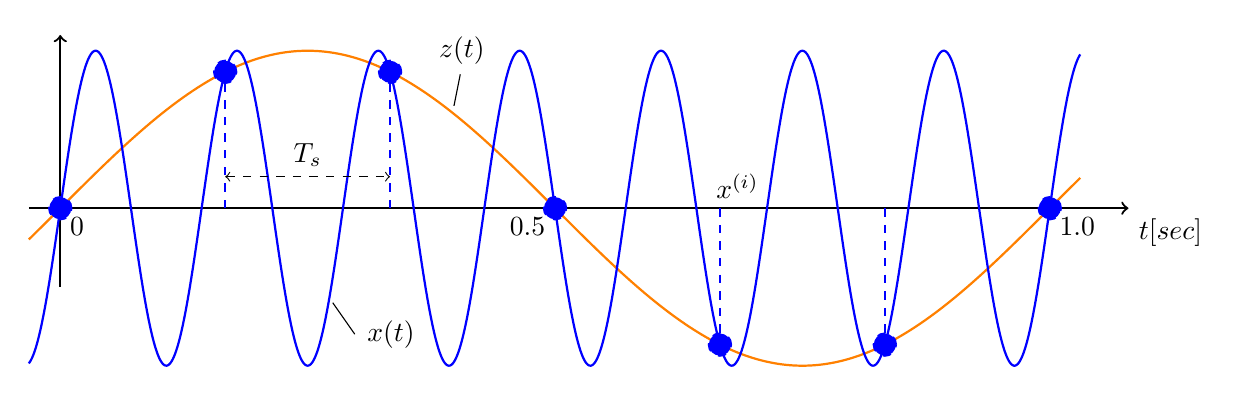
\begin{tikzpicture}[scale=2]
  \draw [thick,->](-0.2,0) -- (2*pi+0.5,0) node[below right] {$t [sec]$};
  \draw [thick,->](0,-0.5) -- (0,1.1);
  \draw [domain=-0.2:2*pi+0.2,samples=1000,orange, thick] plot(\x,{sin(\x r)});
  \draw [domain=-0.2:2*pi+0.2,samples=1000,blue, thick] plot(\x,{sin(7*\x r)});  
  \draw [domain=0:2*pi, samples=7, ycomb, mark=*,blue, dashed, thick] plot(\x,{sin(\x r)});
  \node at (2.55,1) {$z(t)$};
  \draw (2.54,0.85) -- (2.5,0.65);
  \node at (2.1,-0.8) {$x(t)$};
  \draw (1.87,-0.8) -- (1.73,-0.6);
  \node at (4.3,0) [above] {$x^{(i)}$};
  \node at (2*pi,0) [below right] {$1.0$};
  \node at (pi,0) [below left] {$0.5$};
  \node at (0,0) [below right] {$0$};
  \draw [<->, thin, dashed] (pi/3,0.2) -- (pi/2,0.2) node[above] {$T_s$} --(2*pi/3,0.2);
\end{tikzpicture}
\caption[Illustration of Nyquist Sampling]{Illustration of the Shannon/Nyquist Sampling Theorem. The blue curve is the original signal $x(t)$ which is a sinusoid with frequency $f = 7$ Hz. The blue points are discrete samples $x^{(i)}$ taken from $x(t)$ at a sampling rate $f_s = 7$ Hz, which is below the Nyquist Rate $2f = 14$ Hz. Thus, aliasing occurs and interpolation algorithms will reconstruct an alias $z(t)$ (orange curve) of $x(t)$.}
\label{fig:nyquist}
\end{figure}

Suppose we wish to reconstruct $x(t)$ by interpolating the samples.
There is an infinite number of continuous functions that fit this set of samples.
However, it can be shown that only one of them has a bandwidth of no more than $f_s/2$.
Thus, if $f < f_s/2$ (the \emph{Nyquist Criterion}), then $x(t)$ is the unique function that will be approximated by interpolation algorithms such as the \emph{Whittaker-Shannon interpolation formula} \cite{shannon1949}.

In Figure \ref{fig:nyquist}, we have a sinusoidal signal $x(t)$ with frequency $f$.
The sampling rate is $f_s=f$ and therefore below the signal's \emph{Nyquist rate} $2f$. 
Thus, we are unable to reconstruct $x(t)$ from the samples. 
Instead, we will reconstruct an \emph{alias} $z(t)$ which, in this case, is another sinusoid with frequency $f/7$.
The original signal $x$ is lost.

We have illustrated Nyquist sampling in the 1-dimensional case.
The same principles hold for higher dimensional signals such as images and videos.

For signals that vary with space, the sampling rate is governed by the desired spatial resolution.
In order to recover the finer details (the high-frequency components) of an image, we require a higher pixel density (i.e. a larger number of pixels per centimeter (ppcm)).

Nyquist sampling underlies almost all signal acquisition protocols that are found in practice. 
It is the basis of medical imaging, audio and video recording and radio receivers.

\subsection{Signal Compression}
\label{sect:compression}
The sampling theorem imposes a lower bound on the sampling rate above which we are able to perfectly reconstruct the desired signal.
This lower bound is often very high and we end up with a very large number of measurements.
Storage and transfer of such signals becomes prohibitively expensive as the size of the signal grows.
Thus, a need for \emph{data compression} arises.

We will discuss a particular type compression algorithm known as \emph{transform coding}.
It is the standard compression method for a wide range of manmade signals such as audio, photos, and video and is the basis of many common signal formats such as JPEG (images), MPEG (video) and MP3 (audio).

Let $\bm v$ by a real-valued digital signal of length $M$, $\bm v \in \mathbb{R}^M$.
Without loss of generality, $\bm v$ is assumed to be a one-dimensional signal.
If we are working with a multi-dimensional signal, we may first vectorize it into a long vector.
When compressing digital signals, we are usually interested in \emph{lossy compression}.

Any vector in $\mathbb{R}^M$ can be expressed as a linear combination of $M$ \emph{basis vectors} $\bm\psi_j \in \mathbb{R}^M$:
\begin{equation}
\label{eqn:cs-transform1}
  \bm v = \sum_{j=1}^M w_j \bm\psi_j
\end{equation}
where $w_j$ is the coefficient (or weight) associated with $\bm\psi_j$.

By forming the \emph{basis matrix} $\bm\Psi = \left[\bm\psi_1 \,\cdots\, \bm\psi_M\right]$, we can express equation (\ref{eqn:cs-transform1}) in matrix form
\begin{equation*}
\bm v = \bm\Psi \bm w
\end{equation*}
where $\bm w = (w_1,\cdots,w_M)^T$.
For simplicity, we assume that the basis $\bm\Psi$ is orthonormal, so that $\bm\Psi\bm\Psi^T = \bm I_M$ and $\bm\psi_i^T\bm\psi_j$ is 1 if $i = j$ and 0 otherwise.
Thus, the coefficient $w_j$ is given by $w_j = \bm v^T\bm\psi_j$.

We now have two equivalent representations of the same signal, $\bm v$ in the original basis and $\bm w$ in the $\bm\Psi$ basis.
Since $\bm\Psi$ is orthogonal, $\bm v$ and $\bm w$ have the same $\ell_2$-norm, $||\bm v||_2 = ||\bm\Psi\bm w||_2 = ||\bm w||_2$.
However, in the original signal, $\bm v$, the energy is typically spread over many of its components.
On the other hand, it is possible to find a basis $\bm\Psi$ such that the energy of the transformed signal, $\bm w$, is concentrated in only a few large components $w_j$ and a large fraction of its entries are very close to zero.

Suppose that we delete the entries $w_j$ that are very small and replace them with zero to obtain $\bm{\hat w}$.
Let $\bm{\hat v} = \bm\Psi\hat{\bm w}$ the approximate signal in the original domain.
Since $\bm{\hat w}$ is very close to $\bm w$, it follows that
\begin{equation*}
  ||\bm{\hat v} - \bm v||_2 = ||\bm\Psi\bm{\hat w} - \bm\Psi\bm w||_2 = ||\bm\Psi (\bm{\hat w} - \bm w)||_2 = ||\bm{\hat w} - \bm w||_2
\end{equation*}
is very small.

\begin{figure}
  \centering
  \begin{subfigure}[b]{0.4\textwidth}
    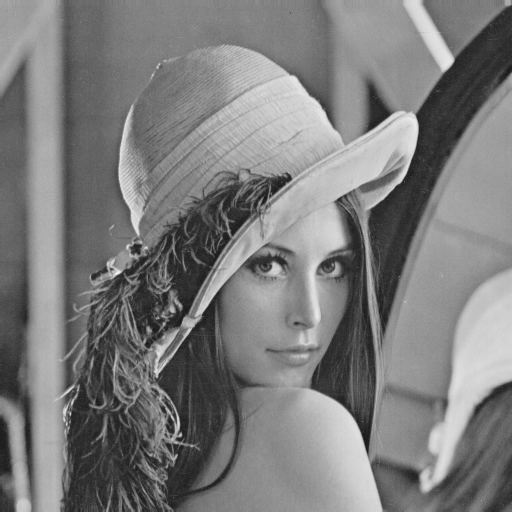
\includegraphics[width=\textwidth]{Chapter2/Images/lenna512.png}
    \caption{Uncompressed Image}
    \label{fig:ch2:lenna_orig}
  \end{subfigure}
  \begin{subfigure}[b]{0.4\textwidth}
    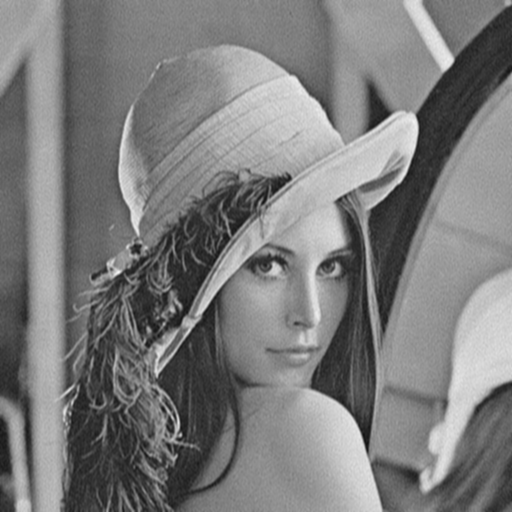
\includegraphics[width=\textwidth]{Chapter2/Images/lenna512_dct.png}
    \caption{Compressed Image via DCT}
    \label{fig:ch2:lenna_dct}
  \end{subfigure}
  \caption[Image Compression using DCT]{The uncompressed image has a resolution of $512\times 512$, i.e. 262,144 pixels. We compress the image by performing a Discrete Cosine Transform (see Section \ref{sect:dct}) and storing only the largest 27,832 coefficients. The compression ratio is 9.42.}
  \label{fig:ch2:dct}
\end{figure}

Thus, a viable method for lossy compression of the signal $\bm v \in \mathbb{R}^M$ would be the following:
\begin{enumerate}
\item Compute the full set of transform coefficients $\{w_j\}_{j=1}^M$ via $\bm w = \bm\Psi^T\bm v$.
\item Locate all the coefficients $w_j$ whose absolute value is above a certain threshold (suppose there are $K$ of them). 
\item Discard all the $(M-K)$ small coefficients
\item Store the values and locations of the $K$ large coefficients
\end{enumerate}
In order to view the compressed signal in the original domain, we reconstruct it via the transform: $\bm\Psi\bm{\hat w} = \bm{\hat v}$, where $\bm{\hat w}$ is $\bm w$ with the $(M-K)$ smallest coefficients replaced by zero.

It is possible to find basis matrices $\bm\Psi$ that result in very high compression ratios for a wide range of signals without any noticable reduction in the signal quality.
Furthermore, many of the commonly used basis transforms can be computed very efficiently.

Audio signals and a wide class of communication signals are highly compressible in the localized Fourier basis.
Images and video signals, on the other hand, can often be compressed via the \emph{Discrete Cosine Transform} (DCT) or the \emph{Discrete Wavelet Transform} (DWT).
For instance, the JPEG standard for image compression is based on the DCT \cite{wallace1992}, while the more modern JPEG2000 format uses the CDF 9/7 wavelet transform or the CDF 5/3 wavelet transform \cite{usevitch2001}.

In Figure \ref{fig:ch2:dct}, we compress the standard test image ``Lenna'' via a DCT. 
We are only storing about 10\% of the transform coefficients.
Yet, the difference between the original image and the compressed image is hardly noticable.

We will discuss the DCT and the DWT in more detail in Chapter \ref{ch:dwt}.

\section{Compressive Sensing}
The conventional approach to data acquisition and compression is very effective and has been highly influential.
However, it is also extremely wasteful.
We acquire a huge amount of data at the signal sampling stage and then proceed to discard a large part of it at the compression stage.

Compressive Sensing \cite{candes2006,donoho2006} is a more general approach that lets us \emph{acquire signals directly in a compressed format}.
This is clearly more efficient as it allows us to skip the intermediate stage of taking $N$ samples.

In this section we will formulate the Compressive Sensing problem.
For simplicity, the focus will be on discrete signals such as digital images or videos.

\subsection{The Compressive Sensing Problem}
Let $\bm v \in\mathbb{R}^M$ be the signal of interest.
As an example, $\bm v$ could be a digital photograph, such as Figure \ref{fig:ch2:lenna_orig}, that has been unrolled into a long vector of length $M$, where $M$ is the number of pixels.

Suppose $\bm v$ is currently unknown and we want to acquire a compressed representation of it without measuring $\bm v$ directly.
To do so, consider the following linear sensing scheme:
We measure inner products between the signal $\bm v$ and a collection of $M$-dimensional vectors $\{\bm\theta_i\}_{i=1}^N$ to obtain the measurements $y_j = \bm v^T\bm\theta_i$ for $i = 1,\cdots,N$. 
This relation can be expressed more succinctly as%Alternatively, we can express equation (\ref{eqn:ch2:sensor1}) as
\begin{equation}
\label{eqn:cs_sensing}
  \bm y = \bm\Theta\bm v
\end{equation}
where $\bm y = (y_1,\cdots,y_N)^T$ and $\bm\Theta$ is the $N\times M$ \emph{sensing matrix} given by
\begin{equation}
\label{eqn:ch2:sensor2}
  \bm\Theta = 
  \begin{bmatrix} 
    \bm \theta_1^T\\
    \vdots\\
    \bm \theta_N^T
  \end{bmatrix}.
\end{equation}

We are interested in the \emph{undersampled} situation where $N < M$.
In particular, we would like to acquire a compressed representation $\bm y$ of $\bm v$ using as few measurements as possible, while still being able to recover the original signal.

There are two problems that stand out at this point. 
\begin{enumerate}
\item Given that $N << M$, how can we ensure that, during the measurement process, we do not lose any information contained in $\bm v$ (i.e. $\bm y$ captures all the information in $\bm v$)?
\item Given our measurements $\bm y$ and knowledge of the sensing matrix $\bm\Theta$, how do we recover the signal of interest $\bm v$?
\end{enumerate}

At an intuitive level, we would expect at least some information to be destroyed during the measurement process, especially if the number of measurements, $N$, is substantially lower than the length of the desired signal, $M$.
Moreover, even if $\bm y$ did contain the same information as $\bm v$, we are still faced with solving the linear system in equation (\ref{eqn:cs_sensing}).
This system is underdetermined and hence there are infinitely many vectors $\bm v$ that satisfy $\bm\Theta\bm v=\bm y$. 

\subsection{Sparse Signals}
In general, we cannot resolve these issues.
However, if we restrict ourselves to a certain class of signals, it is possible to make progress.

In particular, we will focus on signals that have \emph{sparse representations}.
A signal $\bm v \in\mathbb{R}^M$ has a sparse representation if there exists a $M\times M$ basis matrix $\bm\Psi$ so that the transformed signal $\bm w$, where $\bm v = \bm\Psi\bm w$, is \emph{sparse}.

We say that $\bm w$ is \emph{$K$-sparse} if $\bm w$ has $K$ non-zero components.
Equivalently, $\bm w$ is $K$-sparse if 
\footnote{The $\ell_p$-norm of a vector $\bm z \in\mathbb{R}^n$ is defined as follows for $p>0$:
\begin{equation*}
\label{eqn:lp-norm}
  ||\bm z||_p \equiv \left( \sum_{i=1}^n |z_i|^p \right)^\frac{1}{p}.
\end{equation*}
If $p=0$ we can define the $\ell_0$ ``norm'' of $\bm z$ to be the number of its non-zero entries:
\begin{equation*}
\label{eqn:l0-norm}
  ||\bm z||_0 \equiv  \sum_{i=1}^n \mathbbm{1}\{z_j \neq 0\}
\end{equation*}
}
$||\bm w||_0 = K$.

In Section \ref{sect:compression} we noted that many manmade signals are compressible.
They have an almost-sparse representation, meaning that, when expressed in the basis $\bm\Psi$, almost all of their energy is contained in only $K$ components and the remaining components are very close to zero.
Such signals are well-approximated by $K$-sparse representations.

\section{Solving the Compressive Sensing Problem}
So let us suppose then, that the desired signal $\bm v$ is $K$-sparse when expressed in the $\bm\Psi$ basis, where $K$ is 
small ($K << M$).
We can substitute $\bm v = \bm\Psi\bm w$ into (\ref{eqn:cs_sensing}) to get
\begin{equation*}
  \bm y = \bm\Theta\bm v = \bm\Theta\bm\Psi\bm w
\end{equation*}

Let us define $\bm\Phi = \bm\Theta\bm\Psi$, so that
\begin{equation}
  \label{eqn:cs}
  \bm y = \bm\Phi\bm w .
\end{equation}
We have arrived at another underdetermined linear system.
The CS measurements $\bm y$ are still the same as in (\ref{eqn:cs_sensing}), but the sensing matrix $\bm\Theta$ has been replaced by the new sensing matrix $\bm\Phi$.

However, we now want to recover the signal $\bm w$ and we can use the fact that $\bm w$ is $K$-sparse for some $K$.
This allows us to address the problems above.

The information in $\bm w$ is highly localized.
It is fully contained in only $K << M$ of its entries.
Thus, as long as $N\geq K$, it should, at least in principle, be possible for a measurement vector $\bm y$ of length $N<<M$ to completely capture the information within $\bm w$.

Furthermore, since $(M-K)$ entries of $\bm w$ are zero, it follows that in (\ref{eqn:cs}), $\bm y$ is actually linear combination of only $K$ columns of $\bm\Phi$. 
So, if $N\geq K$, we might expect to find suitable constraints that allow us to recover $\bm w$.
Once $\bm w$ is recovered, we can compute $\bm v$ via $\bm v = \bm\Psi\bm w$.

\subsection{Constructing the Sensing Mechanism}
\label{sect:sensors}
In practice, we do not know the locations of the $K$ nonzero entries in $\bm w$.
So the first challenge in a compressive sensing system is to design a $N\times M$ sensing matrix $\bm\Theta$ which ensures that, for any signal $\bm v$ that has a $K$-sparse representation in the basis $\bm\Psi$, we measure all the essential information in the signal.

We will not go into the theoretical details of designing an optimal CS measurement process. Instead we will refer the reader to \cite{candes2008} and simply state three particular sensing matrices that have been used successfully in practice:
\begin{enumerate}
\item Form $\bm\Theta$ by sampling its entries $\theta_{ij}$ independently from the Gaussian distribution with mean zero and variance $1/M$: $\theta_{ij}\, \stackrel{iid}{\sim}\, \mathcal{N}(0,1/M)$.
\item Sample the entries $\theta_{ij}$ independently from a symmetric Bernoulli distribution, $P(\theta_{ij} = \pm 1/\sqrt{M}) = 1/2$. 
\item Form $\bm\Theta$ by starting with the $M\times M$ identity matrix $I_M$ and deleting $M-N$ of its rows at random. This sensing matrix corresponds to measuring a down-sampled version of the signal $\bm v$ directly. If the signal of interest $\bm v$ is a digital image, then $\bm\Theta$ measures $\bm v$ after an \emph{image mask} has been applied to it. This sensing mechanism has been succesfully used in \cite{pilikos2014}.
\end{enumerate}

\subsection{Signal Recovery}
Using the sensing mechanisms outlined above, we are able to measure the signal $\bm v$ directly in a compressed format $\bm y$.
The final part of a Compressive Sensing system is a signal reconstruction algorithm that decompresses $\bm y$ and recovers $\bm v$ or, equivalently, its sparse representation $\bm w$.

This can be achieved by searching for the sparsest solution $\bm w$ that satisfies equation (\ref{eqn:cs}) \cite{baraniuk2007}.
That is, the desired signal is the solution to the optimization problem:
\begin{equation}
\label{eqn:cs_l0}
  \min_{\bm w} ||\bm w||_0 \qquad \mbox{subject to} \qquad \bm\Phi\bm w = \bm y
\end{equation}
Unfortunately, (\ref{eqn:cs_l0}) is an NP-complete problem that can only be solved by an exhaustive search through all possible combinations for the locations of the non-zero entries in $\bm w$.

Luckily, and somewhat surprisingly, it can be shown that, if $N = O(K\log(M/K))$, it is possible to reconstruct $K$-sparse signals exactly by solving the $\ell_1$-optimization problem \cite{baraniuk2007,candes2008}
\begin{equation}
\label{eqn:cs_l1}
  \min_{\bm w} ||\bm w||_1 \qquad \mbox{subject to} \qquad \bm\Phi\bm w = \bm y
\end{equation}
The solution $\bm{\hat w}$ can be transformed to the original domain via $\bm{\hat v} = \Psi\bm{\hat w}$.

In practice, signals $\bm v$ usually only have an almost-sparse representation.
Thus, the reconstruction is not completely exact and the solution $\bm{\hat v}$ will be a close approximation to $\bm v$.

A large part of the CS literature is focused on developing algorithms that recover a signal $\bm v$ from a set CS measurement $\bm y$, either by solving (\ref{eqn:cs_l1}) or through some alternative route.

For a discussion and comparison of some of the most widely used algorithms, see \cite{pilikos2014}.

In Chapter \ref{ch:msce} we will approach the CS signal reconstruction problem in a Bayesian way.
Before we do so, however, we need to introduce the Sparse Bayesian Learning framework (Chapter \ref{ch:rvm}) and provide a more thorough discussion about basis functions (Chapter \ref{ch:dwt}).


\chapter{Basis Functions}
\label{ch:dwt}

%\item Explain MSE, PSNR
In Section \ref{sect:compression}, we introduced transform coding.
We said that any discrete signal $\bm v \in \mathbb{R}^M$ can be expressed in a different basis via a basis transform:
\begin{equation*}
  \bm v = \bm\Psi\bm w
\end{equation*}
where $\bm\Psi$ is the $M\times M$ basis matrix and $\bm w \mathbb{R}^M$ is the representation of $\bm v$ in the $\bm\Psi$ basis.

The particular classes of signals $\bm v$ that we are interested in are digital images and digital video.
The aim of this chapter is to construct a basis matrix $\bm\Psi$ that gives us a (near-) sparse representation of a wide range of such signals $\bm v$.
Finding a set of basis functions $\bs\Psi$ that achieve such a transformation lies at the heart of many lossy compression techniques.

It is important to note here that the choice of basis functions $\bs \Psi$ typically has a significant effect on the performance of the reconstruction algorithms.

\section{Discrete Cosine Transform}
The first basis transform that we will use is the Discrete Cosine Transform (DCT), one of the most widely used transforms in signal processing.
It underlies JPEG image compression and is used in various video compression algorithms such as MJPEG, MPEG, H.261 and H.263 \cite{zeng2013}.
\footnote{A related transform, known as the \emph{Modified DCT} is used in many lossy audio compression formats such as MP3, AAC and Vorbis.}

A DCT decomposes a signal in terms of cosine functions with different frequencies.
Its extensive use in lossy compression algorithms is due to the DCT's \emph{energy compaction} properties.
The majority of a signal's energy is contained within relatively few coefficients - typically those corresponding to the lower frequency basis functions.

On a side note, the DCT comes in a various versions that have minor differences between them.
In the following, we will describe the most widely used version, known as the \emph{DCT-II}, as well as its inverse transform, the \emph{DCT-III}.
We will refer to them simply as ``the DCT'' and ``the Inverse DCT (IDCT)'', respectively.

\subsection{One-Dimensional DCT}
\begin{figure}
  \centering
  \begin{subfigure}{0.45\textwidth}
    \centering
    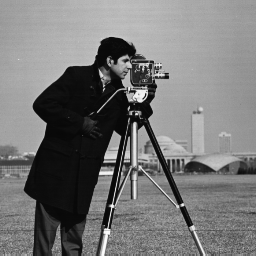
\includegraphics[width=\textwidth]{Chapter3/Images/cameraman.png}
    \caption{Original signal $\bm v$}
  \end{subfigure}
  \begin{subfigure}{0.45\textwidth}
    \centering
    
\includegraphics[width=\textwidth]{Chapter3/Images/dctCoeff.png}
    \caption{DCT of $\bm v$}
  \end{subfigure}
  \caption{Panel (a) shows the original signal $\bm v$, a 256$\times$256 grayscale image known as ``cameraman''. Panel (b) illustrates the 2-D DCT of $\bm v$. The brightness of a an element increases with the absolute value of the corresponding DCT coefficient. (The high-frequency coefficients have been enhanced to show more detail).}
  \label{fig:ch3:dct}
\end{figure}

Formally, the DCT $\bm w$ of a one-dimensional signal $\bm v$ of length $M$ is given by
\begin{equation}
  w_k = c(k) \sum_{m=1}^{M} v_m \, \cos\left(\frac{\pi(2i-1)(k-1)}{2M}\right) \qquad k = 1,\cdots,M
\end{equation}
where
\begin{equation*}
  c(k) = \left\{\begin{array}{ll}
  \sqrt{\frac{1}{M}} & \qquad\mbox{if $k=1$}\\
  \sqrt{\frac{2}{M}} & \qquad\mbox{otherwise}\\
  \end{array}\right.
\end{equation*}
This transforms a signal $\bm v$ in the original domain (time or space) into its representation $\bm w$ in the DCT domain.

\begin{figure}
  \centering
  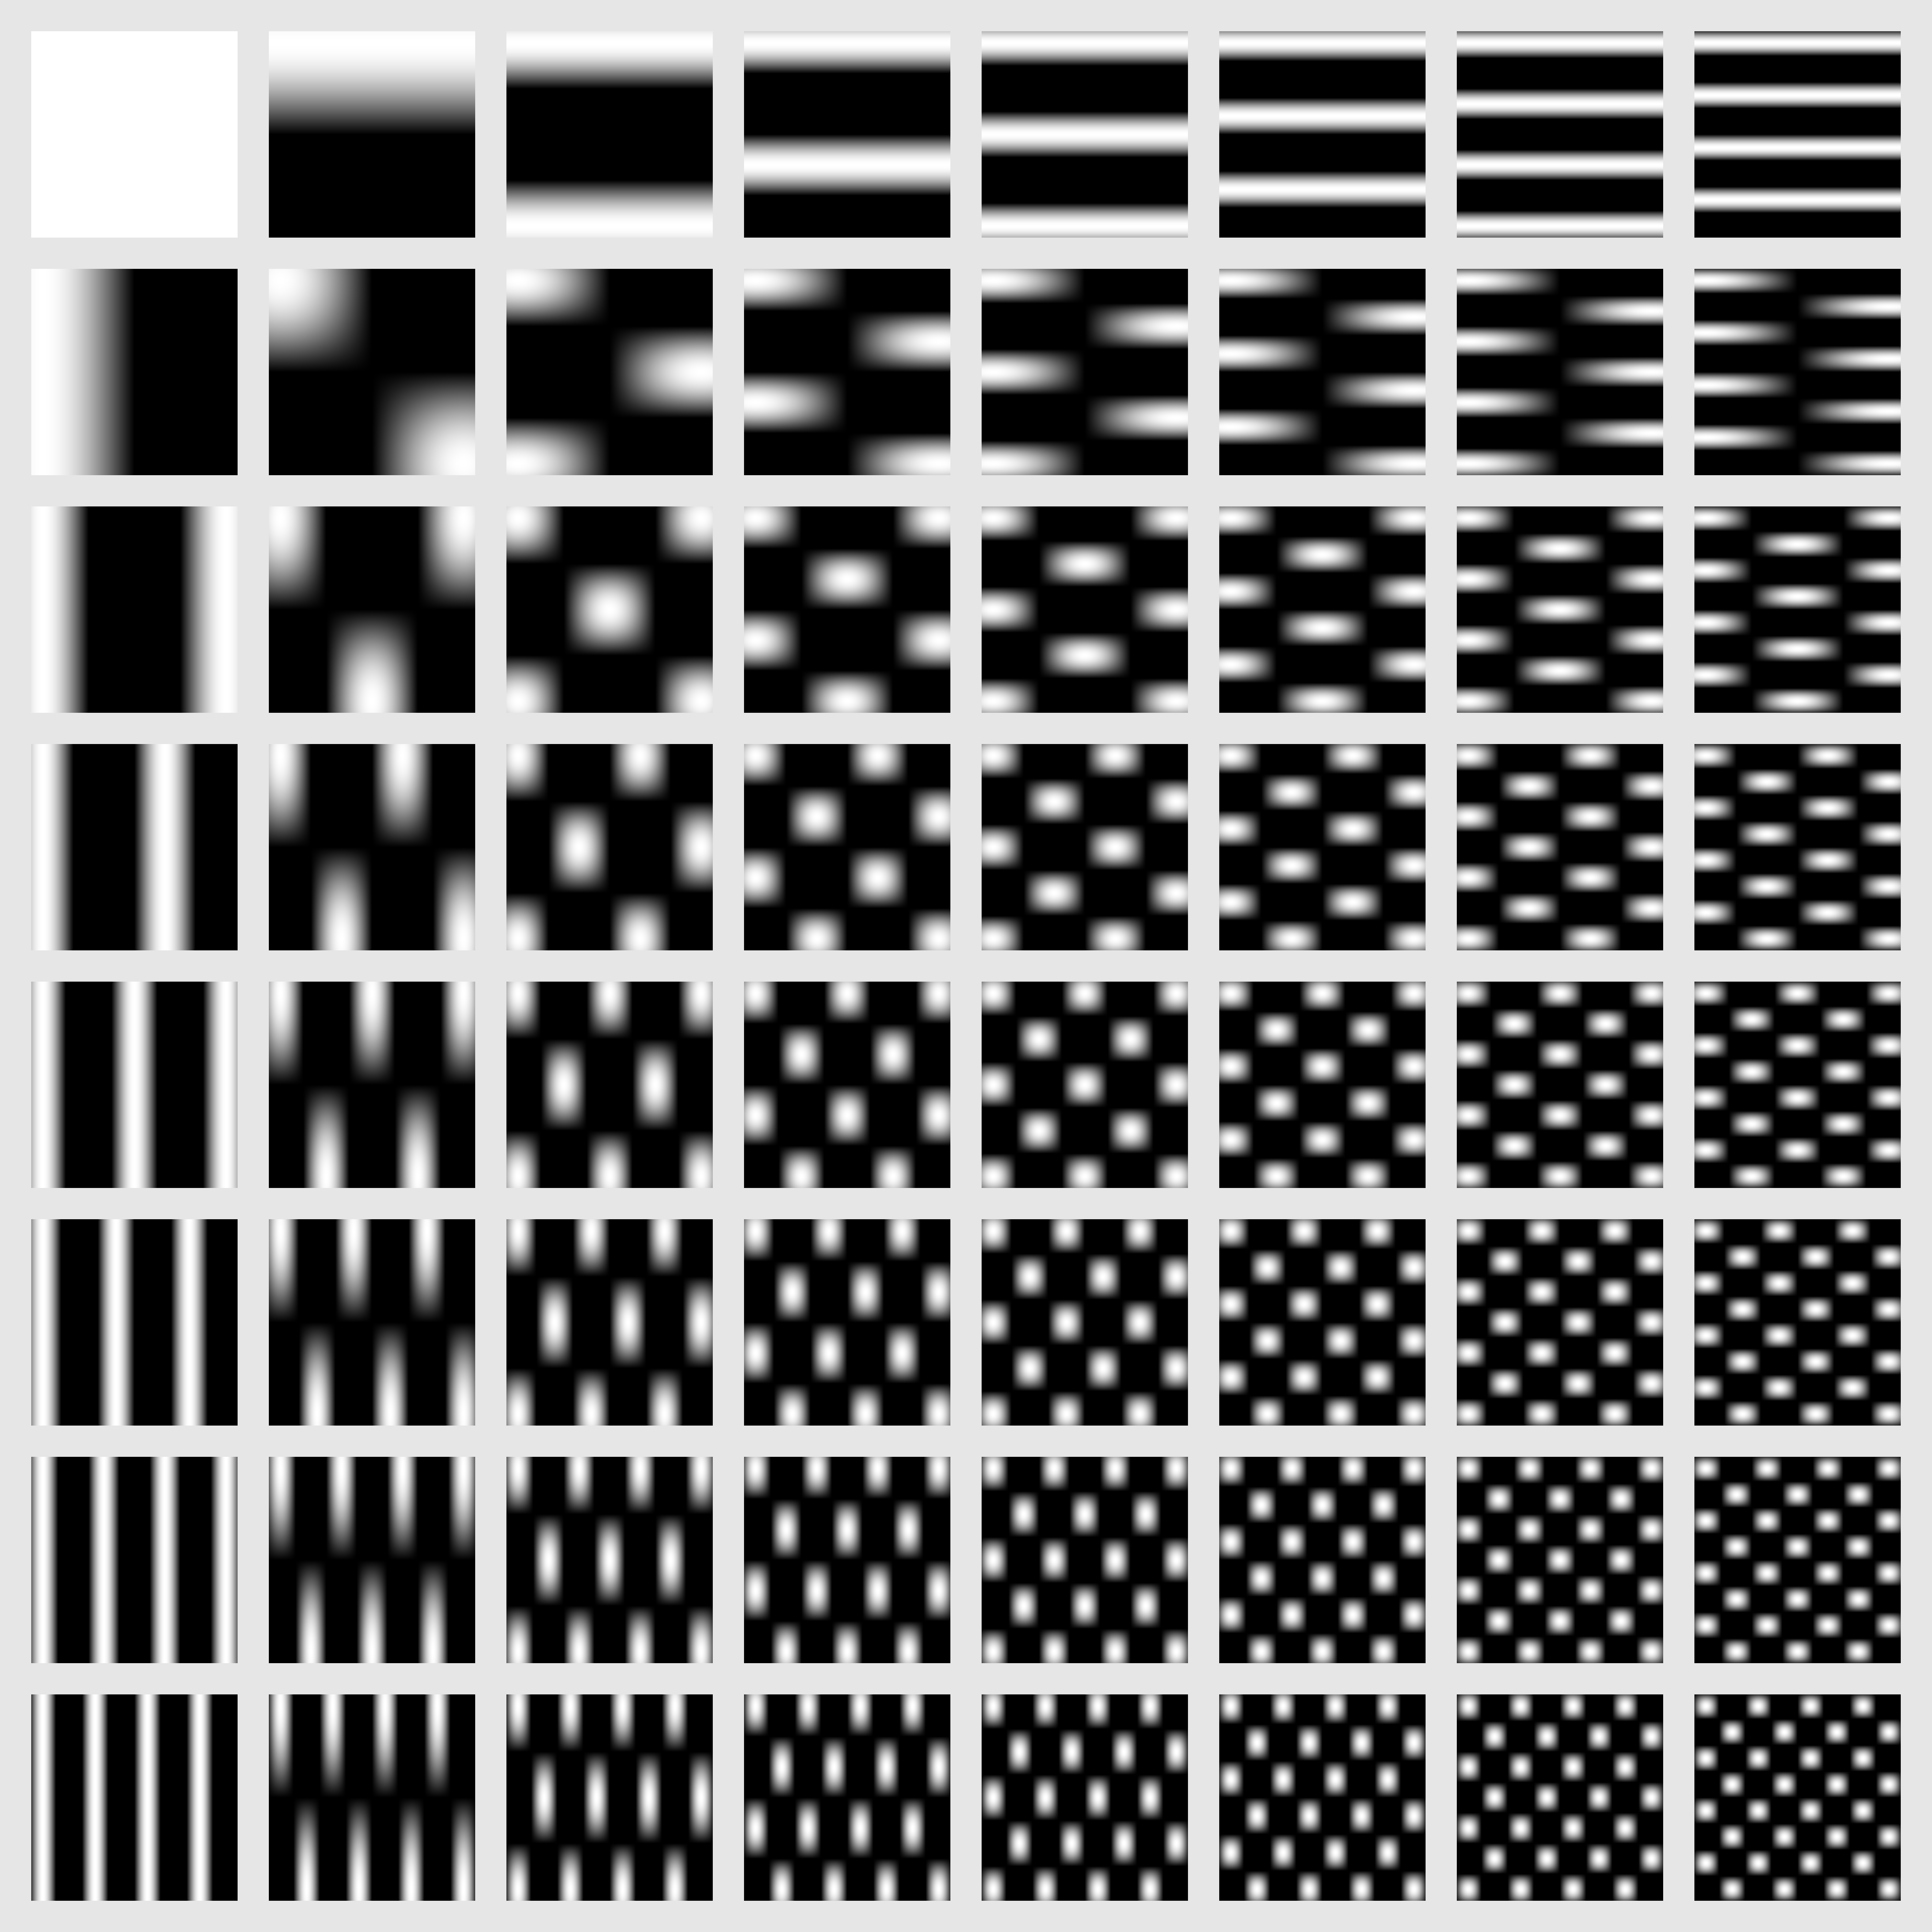
\includegraphics[width=0.5\textwidth]{Chapter3/Images/dct2functions.png}
  \caption{The 2-D DCT basis functions that are used by the DCT to decompose a $8\times 8$ image. 
    The spatial frequency increases towards the bottom right corner.}
  \label{fig:2D-DCT}
\end{figure}

Conversely, given a signal $\bm w$ in the DCT domain, we can transform it back to the orignal (time or space) domain via the IDCT defined by
\begin{equation}
  \label{eqn:idct}
  v_n = \sum_{k=1}^M c(k) w_k  \, \cos\left(\frac{\pi(2i-1)(k-1)}{2M}\right) \qquad n = 1,\cdots,M
\end{equation}

We can express equation (\ref{eqn:idct}) in the desired form $\bm v=\bm P\bm w$.
The entries of the basis matrix $\bm P$ are given by
\begin{equation}
  P_{n,k} = c(k)\, \cos\left(\frac{\pi(2i-1)(k-1)}{2M}\right).
\end{equation}
Note that the basis matrix $\bm P$ is orthogonal, $\bm P^T\bm P=\bm I_M$.

\subsection{Multi-Dimensional DCT}
Once we know how to perform the DCT on a one-dimensional signal, we can easily extend the transform to multi-dimensional signals (images, video, etc).
To do so, we simply perform successive 1-D transforms along each dimension of the signal.
This property is known as \emph{seperability}.

Suppose the signal of interest is a digital image.
That means that $\bm v$ is a $M_1\times M_2$ matrix where $M_1\times M_2$ is the resolution of the image.
To transform the signal, we first perform the DCT on every row of the matrix.
Following that, we perform the DCT on every column of the resulting matrix to get the final transformed signal.

Figure \ref{fig:ch3:dct} shows an example of a 2-D signal $\bm v$ and its transform $\bm w$.
Note that the majority of the energy of the transformed signal is concentrated in the top left corner.
Most of the DCT coefficients are zero or very close to zero.

In Figure \ref{fig:2D-DCT}, we show the 2-D basis functions that would used by the DCT to decompose a signal of size $8\times 8$.
Each basis function is characterised by a horizontal and vertical spatial frequency.
Typically, natural images are mostly made up of low-frequency components and the corresponding coefficients are therefore relatively large.
The highest-frequency components are usually only needed to describe very fine details.

The DCT can be used to decompose video signals with 3-D basis functions. 
Besides the spatial frequencies, the 3-D basis functions have an additional temporal frequency component.
To perform the DCT on a video, we could first perform the 2-D DCT on every frame of the video followed by a 1-D DCT across the temporal axis for each pixel.

For a discussion on the properties of the DCT, see \cite{khayam2003}

\section{Discrete Wavelet Transform}
Wavelets have become a very popular tool in signal processing.
Their energy compaction properties are on par and often superior to those of the DCT for a wide range of signal classes.
In 2000, the JPEG committee released a new image coding standard, JPEG2000, that is gradually replacing the original JPEG standard.
The new format moved away from the DCT and uses a Discrete Wavelet Transform (DWT) instead.

[CAVEAT and INTRO]

\subsection{Introduction to Wavelets}
To motivate wavelets, consider again the one-dimensional signal $\bm v$ of length $M$.
Suppose, for simplicity, that $M$ is a power of $2$, $M = 2^q$ say.
We can view the $\bm v$ as a piecewise-constant function $v(x)$ on the half-open interval $[0,1)$, where $v(x) = v_i$ if $x \in [\frac{i-1}{M}, \frac{i}{M})$.

Let $V^j$ denote the vector space containing all piecewise-constant functions $f$ defined on the interval $[0,1)$ that consist of $2^j$ pieces, each of which is constant across a sub-interval of size $2^{-j}$.
Thus, $V^0$ consists of all functions that are constant on $[0,1)$, while $V^1$ consists of all functions that have two constant pieces, one over $[0,1/2)$ and one over $[1/2,1)$.
In particular, our signal $v(x)$ resides in the space $V^q$.

Note that if $f \in V^j$, then $f \in V^{j+1}$.
Thus, the vector spaces $V^j$ are nested: $V^0 \subset V^1 \subset V^2 \subset \cdots$.

Next, we need to choose a basis for each vector space $V^j$.
To do so, we introduce a \emph{scaling function} (also known as \emph{scalet}, or \emph{father wavelet}) that is usually denoted $\phi(x)$.
The form of the scaling function depends on the particular choice wavelet decomposition.

\begin{figure}
  \centering
  \begin{subfigure}{0.4\textwidth}
    \centering
    \begin{tikzpicture}[xscale=2]
      \draw [thin,->] (0,-1.5) -- (0,1.5);
      \draw [thin,->] (-0.5,0) -- (1.5,0) node[below]{\small$x$};
      \draw [very thick] (-0.2,0) -- (0,0) node[below left]{\small$0$} -- (0,1) node[left]{\small$1$} -- (1,1) -- (1,0) node[below]{\small$1$} -- (1.3,0);
    \end{tikzpicture}
    \caption{Haar scaling function $\phi(x)$}
    \label{fig:haar_scaling}
  \end{subfigure}
  \begin{subfigure}{0.4\textwidth}
    \centering
    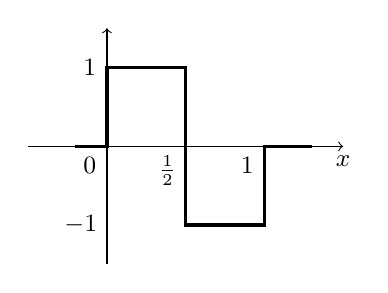
\begin{tikzpicture}[xscale=2]
      \draw [thin,->] (0,-1.5) -- (0,1.5);
      \draw [thin,->] (-0.5,0) -- (1.5,0) node[below]{\small$x$};
      \draw [very thick] (-0.2,0) -- (0,0) node[below left]{\small$0$} -- (0,1) node[left]{\small $1$} -- (0.5,1) -- (0.5,-1) -- (1,-1) -- (1,0) node[below left]{\small $1$} -- (1.3,0);
      \node at (0,-1)[left]{\small$-1$};
      \node at (0.5,0)[below left]{\small $\frac{1}{2}$};
    \end{tikzpicture}
    \caption{Haar mother wavelet $\psi(x)$}
    \label{fig:haar_mother}
  \end{subfigure}
  \caption{The scaling function and wavelet function for the Haar wavelets.}
  \label{fig:haar_1d}
\end{figure}

For example, for the \emph{Haar wavelets} the scaling function is given by
\begin{equation}
  \label{eqn:haar_scale}
  \phi(x) = \left\{ \begin{array}{rl}
    1& \qquad \mbox{if $0\leq x < 1$}\\
    0& \qquad \mbox{otherwise}
  \end{array}\right.
\end{equation}
See Figure \ref{fig:haar_scaling} for a plot of $\phi(x)$.

Given the scaling function $\phi(x)$, we can define the following basis for $V^j$:
\begin{equation*}
  \phi_k^j(x) := 2^{j/2}\phi(2^j x-k) \qquad k = 0,\cdots, 2^j-1
\end{equation*}

Using this basis, we can decompose our signal $v(x)\in V^q$ as 
\begin{equation*}
  v(x) = \sum_{k=0}^{2^q-1} c_k^q \phi_k^q(x)
\end{equation*}
For the scaling function defined in equation (\ref{eqn:haar_scale}), we have that $c_k^q = v_{k+1}$.

To obtain \emph{wavelets}, consider the \emph{orthogonal complement} of $V^j$ in $V^{j+1}$ and denote it $W^j$. 
That is, $W^j = \{f \in V^{j+1} :\quad \langle f,g\rangle = 0\quad \forall g \in V^j\}$ where the inner product $\langle f,g\rangle$ is given by
\begin{equation*}
  \langle f,g\rangle = \int_0^1f(x)g(x)dx.
\end{equation*}
By forming a basis for $W^j$, we obtain a set of \emph{wavelet functions} $\{\psi_k^j,\, k=0,\cdots,2^j-1\}$.
Wavelet functions can be constructed by scaling and shifting a so-called \emph{mother wavelet} $\psi(x)$ as follows:
\begin{equation*}
  \psi_k^j(x) = 2^{j/2}\psi(2^j x - k) \qquad k = 0,\cdots, 2^j-1
\end{equation*}

For the Haar wavelets, the mother wavelet is given by:
\begin{equation*}
  \psi(x) = \left\{\begin{array}{rl}
  1&\qquad 0 \leq x < 1/2\\
  -1&\qquad 1/2 \leq x < 1\\
  0&\qquad\mbox{otherwise}
  \end{array}\right.
\end{equation*}
The Haar mother wavelet is shown in Figure \ref{fig:haar_mother}.

Note that, since the scaling functions $\phi_k^j$ form a basis of $V^j$ and the wavelet functions $\psi_k^j$ form a basis of $W^k$, and since $W^j$ is the orthogonal complement to $V^j$ in $V^{j+1}$, it follows that the set $\{\phi_k^j, \psi_k^j: k=0,\cdots,2^j-1\}$ forms a basis of the vector space $V^{j+1}$.

This allows us to express our signal $v \in V^q$ as 
\begin{equation*}
  v(x) = \sum_{k=0}^{2^{q-1}-1} d_k^{q-1}\psi_k^{q-1}(x) + \sum_{k=0}^{2^{q-1}-1} c_k^{q-1}\phi_k^{q-1}(x)
\end{equation*}
This gives us the first level of the discrete wavelet transform of $v$.
The coefficients $c_k$ and $d_k$ are sometimes referred to as ``approximation'' coefficients and ``detail'' coefficients, respectively.

We can continue the decomposition by splitting the basis for $V^{q-1}$ into the bases for $V^{q-2}$ and $W^{q-2}$ to get the next level of the transform:
\begin{equation*}
  v(x) = \sum_{k=0}^{2^{q-1}-1} d_k^{q-1}\psi_k^{q-1}(x) + \sum_{k=0}^{2^{q-2}-1} d_k^{q-2}\psi_k^{q-2}(x) + \sum_{k=0}^{2^{q-2}-1} c_k^{q-2}\phi_k^{q-2}(x)
\end{equation*}
To get the full decomposition, we continue in this fashion up to the $q$th level:
\begin{equation*}
  v(x) = \sum_{j=0}^{q-1} \sum_{k=0}^{2^j-1} d_k^{j} \psi_k^j(x) + c_0^0\phi(x)
\end{equation*}
The full DWT of $\bm v$ consists of the coefficients $\{c_0^0, d_k^j:\,j=0,\cdots,q-1, \, k=0,\cdots,2^j-1\}$.


\subsection{Computing the DWT}

\begin{figure}
  \centering
  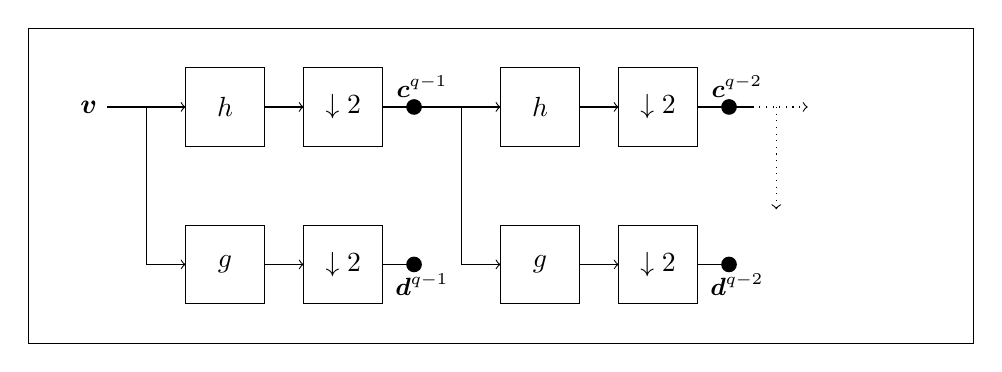
\begin{tikzpicture}
    \draw (0,0) rectangle (12,4);
    \draw (1,3) node[left]{$\bm v$} -- (1.5,3);
    \draw (1.5,1) -- (1.5,3);
    \draw [->](1.5,3) -- (2,3);
    \draw [->](1.5,1) -- (2,1);
    \draw (2,2.5) rectangle (3,3.5);
    \node at (2.5,3) {$h$};
    \draw (2,0.5) rectangle (3,1.5);
    \node at (2.5,1) {$g$};
    \draw [->](3,1) -- (3.5,1);
    \draw (3.5,0.5) rectangle (4.5,1.5);
    \node at (4,1) {$\downarrow 2$};
    \draw (4.5,1) -- (5,1) node [below] {\small$\bm d^{q-1}$};
    \node at (4.9,1)[shape=circle, fill=black, inner sep=2pt, minimum size=2pt] {};
    \draw [->](3,3) -- (3.5,3);
    \draw (3.5,2.5) rectangle (4.5,3.5);
    \node at (4,3) {$\downarrow 2$};
    \draw [->](4.5,3) -- (6,3);
    \draw [->](5.5,3) -- (5.5,1) -- (6,1);
    \node at (5,3) [above] {\small$\bm c^{q-1}$};
    \node at (4.9,3) [shape=circle, fill=black, inner sep=2pt, minimum size=2pt] {};
    \draw (6,2.5) rectangle (7,3.5);
    \node at (6.5,3){$h$};
    \draw (6,0.5) rectangle (7,1.5);    
    \node at (6.5,1){$g$};
    \draw [->] (7,3) -- (7.5,3);
    \draw (7.5,2.5) rectangle (8.5,3.5);
    \node at (8,3) {$\downarrow 2$};
    \draw [->] (7,1) -- (7.5,1);
    \draw (7.5,0.5) rectangle (8.5,1.5);
    \node at (8,1) {$\downarrow 2$};
    \draw (8.5,1) -- (9,1) node [below] {\small$\bm d^{q-2}$};
    \node at (8.9,1) [shape=circle, fill=black, inner sep=2pt, minimum size=2pt] {};
    \draw (8.5,3) -- (9.2,3);
    \draw [->,dotted](9.2,3) -- (9.9,3);
    \draw [->,dotted](9.5,3) -- (9.5,1.7);
    \node at (8.9,3) [shape=circle, fill=black, inner sep=2pt, minimum size=2pt] {};
    \node at (9,3) [above] {\small$\bm c^{q-2}$};
  \end{tikzpicture}
  \caption{The first two levels of the DWT of the signal $\bm v$ of length $2^q$ via a filter bank.}
  \label{fig:filterbank}
\end{figure}

In practice, we can compute one level of the DWT coefficients by passing the signal $\bm v$ through a \emph{low-pass filter} $\bm h$ and a high-pass filter $\bm g$, respectively, and then downsampling the results by a factor of two.
Overall, these computations can be done by multiplying the vector $\bm v$ by a matrix $\bm H$ and a matrix $\bm G$ to get the approximation and detail coefficients, repectively.

To compute the next level, we take the approximation coefficients of the current stage and pass them again through the filter bank.
The procedure is depicted in Figure \ref{fig:filterbank}.




%% The simplest wavelet basis transformation is based on the Haar wavelets.
%% Figure \ref{fig:haarlenna} vizualises a basis transformation of the original image $\bs x$ to $\bs w$. 
%% This example uses a Haar wavelet basis at the first scale.
%% We will explain the Haar wavelet transformations of images and videos in more detail in the next chapter.
%% Dark areas correspond to small coefficients.
%% Note that most entries in $\bs w$ are near zero. 
%% In practice, we approximate these entries as zero and treat $\bs w$ as sparse.

%% \begin{figure}
%% \center
%% 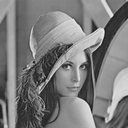
\includegraphics{Images/128.png}
%% 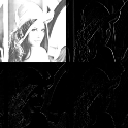
\includegraphics{Images/haar.png}
%% \caption{Original image $\bs x$ (left) and its Haar basis transformation $\bs w$ (right). See next chapter for more details on Haar wavelets.}
%% \label{fig:haarlenna}
%% \end{figure}

%% \section{Haar basis functions}
%% The RVM takes as input a target vector ($\bs y$) and a basis matrix ($\bs \Psi$). 
%% In this respect, it is agnostic about whether the signal is an image or video or of some other type alltogether.
%% Most of this information is encoded in the basis matrix $\bs \Psi$.
%% It is therefore important, and often challenging, to select a good set of basis functions.

%% Our current implementation uses 3-dimensional Haar wavelet basis functions.
%% I will show how the basis matrix $\bs\Psi$ is constructed by briefly describing how the discrete Haar wavelet transform is performed on 1D, 2D and finally on 3D signals.
%% \subsection{1D Haar wavelet transform}
%% Consider a 1-dimensional signal $\bs s = \{s_1,\dots,s_r\} \in \mathbb{R}^r$ ($r$ for ``rows''), where, for simplicity, we assume that $r$ is a power of 2.
%% The Haar wavelet transform can be performed at various resolution scales.
%% The transform at the first scale is given by:
%% \begin{equation*}
%% \bs s = \{s_1,\dots,s_r\}\to \frac{1}{\sqrt{2}}\{s_1+s_2,s_3+s_4,\dots,s_{r-1}+s_r,s_1-s_2,\dots,s_{r-1}-s_r\}=\hat{\bs s}^{(1)}
%% \end{equation*}
%% The first half of the signal is replaced by scaled averages of adjacent elements and the second half is replaced by scaled differences of adjacent elements.
%% By performing this transform again on the first half of $\hat{\bs s}^{(1)}$ while keeping the second half fixed, we get the Haar wavelet transform at the second scale $\hat{\bs s}^{(2)}$. 
%% To get the third scale transform $\hat{\bs s}^{(3)}$, we perform the initial transform on the first quarter of $\hat{\bs s}^{(2)}$ while keeping the rest of the signal fixed.
%% We may continue this process until we reach the $i$th scale, where $2^i = r$.

%% From here on, we will only consider the first scale transform $\hat{\bs s}^{(1)}$ and we will omit the $(1)$ superscript.
%% We can express the transform as a multiplication by an orthogonal $r\times r$ matrix $W$ given by
%% \begin{equation}
%% W = \begin{bmatrix}
%%   \Phi_r \\
%%   \Psi_r \\
%% \end{bmatrix}
%% \end{equation}
%% where $\Phi_r$ and $\Psi_r$ are $(r/2)\times r$ matrices\footnote{Note that the matrix $\Psi_r$ used here is different to the matrix $\Psi$ that was used in the previous chapter (which corresponds to $W^T$ here).} given by
%% \begin{equation*}
%% \Phi_r = \frac{1}{\sqrt{2}} \begin{pmatrix}
%% 1&1&0&0&\cdots&0&0\\
%% 0&0&1&1&\cdots&0&0\\
%% \vdots&\vdots&\vdots&\vdots&\ddots&\vdots&\vdots\\
%% 0&0&0&0&\cdots&1&1
%% \end{pmatrix}
%% \end{equation*}
%% and 
%% \begin{equation*}
%% \Psi_r = \frac{1}{\sqrt{2}} \begin{pmatrix}
%% 1&-1&0&0&\cdots&0&0\\
%% 0&0&1&-1&\cdots&0&0\\
%% \vdots&\vdots&\vdots&\vdots&\ddots&\vdots&\vdots\\
%% 0&0&0&0&\cdots&1&-1
%% \end{pmatrix}
%% \end{equation*}


%% In the signal processing literature, $\Phi_r$ is referred to as a low pass filter, while $\Psi_r$ is referred to as a high pass filter.
%% $\Phi_r$ outputs an average of the signal and $\Psi_r$ outputs the details of the signal.

%% \subsection{2D Haar wavelet transform}
%% Let $A \in \mathbb{R}^{r\times c}$ be a 2-dimensional signal (e.g. an image).
%% For simplicity, we will assume that both $r$ and $c$ are powers of 2 (though not necessarily equal).

%% It is simple to obtain $A$'s Haar wavelet transform $\hat{A}$ at the first scale.
%% This is done by first applying the 1-dimensional transform individually to each column of $A$ to obtain a temporary matrix $\hat A_{temp}$.
%% Next, we apply the 1-dimensional haar wavelet transform individually to each row of $\hat A_{temp}$ to obtain $\hat A$.

%% We can again express the transform as a multiplication of matrices:
%% \begin{equation}
%% \label{eqn:2Dtransform}
%% \hat A = \begin{bmatrix}
%%   \Phi_r\\
%%   \Psi_r\\
%% \end{bmatrix}
%% A
%% \begin{bmatrix}
%%   \Phi_c^T & \Psi_c^T\\
%% \end{bmatrix}
%% \end{equation}
%% where $\Phi_r$ and $\Psi_r$ are as before and $\Phi_c$ and $\Psi_c$ are of similar form but each have dimensions $(c/2)\times c$.
%% This is the transform that was used to generate the RHS of Figure \ref{fig:haarlenna}.
%% We note that the high-pass filters essentially detect edges of various orientations in the image.

%% However, as it currently stands, we cannot use this form of the basis transformation for the reconstruction algorithm. Recall that the RVM requires a \emph{vector} of measurements as opposed to a matrix and also that it requires a single basis matrix, not a basis transform as given in (\ref{eqn:2Dtransform}).

%% To do this, we store the 2-dimensional signal $A$ as a long column vector $\bs a$ of length $rc$ by pasting the individual columns of $A$ one after another.
%% The basis transformation of $\bs a$ can then be expressed as 
%% \begin{equation*}
%% \hat{\bs a} = W \bs a
%% \end{equation*}
%% where $W$ is a $rc \times rc $ matrix given by
%% \begin{equation*}
%% W = 
%% \begin{bmatrix}
%% \Phi_c \otimes \Phi_r \\
%% \Phi_c \otimes \Psi_r \\
%% \Psi_c \otimes \Phi_r \\
%% \Psi_c \otimes \Psi_r \\
%% \end{bmatrix}
%% \end{equation*}

%% The symbol $\otimes$ denotes the \emph{Kronecker product}. 
%% The kronecker product $P \otimes Q$ between matrices $P$ and $Q$ with dimensions $m_P \times n_P$ and $m_Q \times n_Q$, respectively,  is defined to be the block matrix
%% \begin{equation*}
%% \begin{bmatrix}
%% p_{1,1} Q & p_{1,2} Q & \cdots & p_{1,n_P} Q \\
%% p_{2,1} Q & p_{2,2} Q & \cdots & p_{2,n_P} Q \\
%% \vdots&\vdots&\ddots&\vdots \\
%% p_{m_P,1} Q & p_{m_P,2} Q & \cdots & p_{m_P,n_P} Q \\
%% \end{bmatrix}
%% \end{equation*}
%% of size $m_Pm_Q \times n_Pn_Q$.

%% \subsection{3D Haar wavelet transform}
%% Let $V \in \mathbb{R}^{r\times c\times s}$ be a 3-dimensional signal such as a video. 
%% $V$ has $r$ rows, $c$ columns and $s$ slices, and we assume that $r$, $c$ and $s$ are all powers of 2. 
%% We may visualize $V$ as a ``volume'' with 2 spacial dimensions and one time dimension corresponding to frames of the video.

%% To obtain the Haar wavelet transform $\hat V$ of $V$, we first perform the 1-dimensional transform individually on each column in every slice of $V$ to get $\hat V_{temp1}$.
%% We then perform the 1D transform on every row in every slice of $\hat V_{temp_1}$ to get $\hat V_{temp_2}$.
%% Finally, we perform the 1D transform across the slices for every row and column to get $\hat V$.

%% However, like in the 2-dimensional case, we need to be able to pass a single vector of coefficients and a single basis matrix to the RVM.
%% To do this, we vectorize $V$ as follows. 
%% First, we vectorize each individual slice of $V$ as before in the 2D case.
%% Then, we stack all these vectors on top each other to get one very long column vector $\bs v$ of length $rcs$.
%% The Haar wavelet transform is given by 
%% \begin{equation*}
%% \hat{\bs v} = W \bs v
%% \end{equation*}
%% where 
%% \begin{equation*}
%% W = 
%% \begin{bmatrix}
%% \Phi_s \otimes \Phi_c \otimes \Phi_r \\
%% \Phi_s \otimes \Phi_c \otimes \Psi_r \\
%% \Phi_s \otimes \Psi_c \otimes \Phi_r \\
%% \Phi_s \otimes \Psi_c \otimes \Psi_r \\
%% \Psi_s \otimes \Phi_c \otimes \Phi_r \\
%% \Psi_s \otimes \Phi_c \otimes \Psi_r \\
%% \Psi_s \otimes \Psi_c \otimes \Phi_r \\
%% \Psi_s \otimes \Psi_c \otimes \Psi_r \\
%% \end{bmatrix}
%% \end{equation*}


%% \subsection{Daubechies Wavelets}
%% \emph{Intuition. Where do the coeffs come from. Matrices. Boundary conditions.}


%% \section{Forming the basis matrix}
%% \emph{1D, 2D, 3D case. Different scales}

%% For a deeper introduction into wavelets see \cite{stollnitz1995}.
%% For more information on wavelet compression techniques, see \cite{devore1992}.




\chapter{Sparse Bayesian Learning}
\label{ch:rvm}
\emph{Sparse Bayesian Learning} \cite{tipping2001} is a general Bayesian framework within supervised Machine Learning. 
It can be applied to both regression and classification tasks.
The \emph{Relevance Vector Machine}, or \emph{RVM}, is a particular specialisation of the Sparse Bayesian Learning model which has identical functional form to the Support Vector Machine (SVM).
However, the RVM comes with a number of key advantages over the SVM. 
The solution produced by a RVM is typically much sparser than the solution by a comparable SVM.
Furthermore, the RVM is a probabilistic model and as such, allows us to estimate error bounds in its predictions.

In this chapter, we will derive the Sparse Bayesian Learning model for regression.
We will summarise both the original inference algorithm \cite{tipping2001} and also the faster ``Sequential Sparse Bayesian Learning Algorithm'' \cite{tipping2003}.

\section{Model Specification}
We are given a data set of $N$ input vectors $\{\bm x^{(i)}\}^N_{i=1}$ and their associated \emph{targets} $\{y^{(i)}\}_{i=1}^N$.
The input vectors live in $D$-dimensional space, $\bm x \in \mathbb{R}^D$.
The targets are real values, $y \in \mathbb{R}$.
\footnote{When using the Sparse Bayesian model for regression, we assume the targets are real-valued.
  It is also possible to use the model for classification in which cased the targets are assumed to be discrete class labels.
}

We model the data using a linearly-weighted sum of $M$ fixed basis functions $\{\phi_j(\cdot)\}_{j=1}^M$ and base our predictions on the function $f(\cdot)$ defined as
\begin{equation} 
  \label{rvm:function}
  f(\bm x; \bm w) = \sum_{j=1}^M w_j \phi_j(\bm x) = \bm w^T \bm \phi(\bm x)
\end{equation}
where $\bm w = [w_1, \dots, w_M]^T$ and $\bm \phi(\cdot) = [\phi_1(\cdot), \dots, \phi_M(\cdot)]^T$.
Using a large number $M$ of non-linear basis functions $\phi_j : \mathbb{R}^D \to \mathbb{R}$ allows for a highly flexible model. 

The \emph{Relevance Vector Machine}, or RVM, is a specialisation of the Sparse Bayesian Learning model in which the basis functions take the form of \emph{kernel functions} 
\begin{equation*}
  \phi_j(\cdot) \equiv K\left(\cdot\,,\,\bm x^{(j)}\right).
\end{equation*}
This defines a basis function for each training data point $\bm x^{(i)}$.
Typically, we also include an additional \emph{bias} term $\phi_0(\cdot) \equiv 1$, so that $M = N+1$.
The RVM has identical functional form to the popular Support Vector Machine (SVM), but superior properties.
It typically gives sparser solutions than the SVM and has the additional advantage of providing confidence measures for its predictions.

However, in the following derivation, we will stick to the case of general basis functions $\phi_j:\mathbb{R}^D\to\mathbb{R}$.
Thus $M$ need not equal $N+1$ and may, in fact, be a lot larger.

To train the model (\ref{rvm:function}), i.e. find values for $\bm w$ that are optimal in some sense, we make the standard assumption that our training data are samples from the model with additive noise:
\begin{equation}
  \label{rvm:lklhd_1}
  \begin{split}
    y^{(i)} &= f(\bm x^{(i)}; \bm w) + \epsilon^{(i)}\\
    &= \bm w^T \bm \phi(\bm x^{(i)}) + \epsilon^{(i)}\qquad i = 1, \dots, N.
  \end{split}
\end{equation}
The errors $\{\epsilon^{(i)}\}_{i=1}^N$ are assumed to be independent samples from a zero-mean Gaussian distribution with variance $\sigma^2$
\begin{equation}
  \label{rvm:error}
  p(\epsilon^{(i)}) = \mathcal{N}(\epsilon^{(i)}\,|\,0, \sigma^2)\qquad i = 1, \dots, N.
\end{equation}

Combining equation (\ref{rvm:lklhd_1}) with equation (\ref{rvm:function}), we may express the model for the complete data using matrix notation:
\begin{equation}
  \label{rvm:lklhd_2}
  \bm y = \bm\Phi \bm w + \bm \epsilon
\end{equation}
where $\bm \epsilon = \left[\epsilon^{(1)}, \cdots, \epsilon^{(N)}\right]^T$.
The $N\times M$ matrix $\bm \Phi$ is known as the design matrix. 
The $i$th row of $\bm \Phi$ is given by $\bm \phi(\bm x^{(i)})^T$.
The $j$th column of $\bm \Phi$ is given by $\bm \phi_j = \left[\phi_j\left(\bm x^{(1)}\right), \cdots, \phi_j\left(\bm x^{(N)}\right)\right]^T$, which is also referred to as the $j$th \emph{basis vector}.
Thus
\begin{equation*}
  \bm\Phi =
  \begin{bmatrix}
    \bm\phi_1 & \cdots & \bm\phi_M
  \end{bmatrix}
  =
  \begin{bmatrix}
    \bm\phi(\bm x^{(1)})^T\\
    \vdots\\
    \bm\phi(\bm x^{(N)})^T
  \end{bmatrix}
\end{equation*}

Combining equation (\ref{rvm:lklhd_2}) and equation (\ref{rvm:error}), we find that the complete data likelihood function is given by
\begin{equation}
  \label{rvm:complete_lk}
  \begin{split}
    p\left(\bm y\,|\,\bm w,\sigma^2\right) &= \mathcal{N}\left(\bm y\,|\,\bm w,\sigma^2 \bm I_M\right)\\
    &= (2\pi\sigma^2)^{-N/2} \exp\left\{-\frac{1}{2\sigma^2}||\bm y - \bm\Phi\bm w||^2\right\}
  \end{split}
\end{equation}
where $\bm I_M$ is the $M\times M$ identity matrix.

So far, we have specified the general linear regression model.
To get to the sparse Bayesian formulation, we define a zero-mean Gaussian prior distribution over the parameters $\bm w$
\begin{equation}
\label{eqn:prior_w}
  p(\bm w\,|\,\bm \alpha) = \prod_{j=1}^M \mathcal{N}\left(w_j\,|\,0,\alpha_j^{-1}\right)
\end{equation}
where $\bm \alpha = \left[\alpha_1,\cdots,\alpha_M\right]^T$ is a vector of $M$ hyperparameters.
It is important to note that each hyperparameter $\alpha_j$ is solely responsible for controlling the strength of the prior of its associated weight $w_j$.
If $\alpha_j$ is large, the prior over $w_j$ is very strongly peaked at zero.
This form of the prior distribution is, more than anything, responsible for the dramatic sparsity in the final model.

To complete the specification, we must define a prior over the noise parameter $\sigma^2$ and the a hyperprior over the hyperparameters $\bm \alpha$.
Following the derivation in \cite{tipping2001}, we use the following Gamma
\footnote{
The Gamma distribution is defined by   
\[
\GammaDist(z\,|\,a,b) = \Gamma(a)^{-1} b^a z^{a-1} \exp(-bz)  \qquad z,a,b > 0
\]
where $\Gamma(.)$ is the Gamma function defined by 
\[
\Gamma(z) = \int_0^\infty t^{z-1} \exp(-t) dt.
\]
} priors
\begin{equation}
\label{eqn:prior_alpha}
  p(\bm\alpha\,|\,a,b) = \prod_{j=1}^M \GammaDist(\alpha_j\,|\,a,b)
\end{equation}
\begin{equation}
\label{eqn:prior_beta}
  p(\beta\,|\,c,d) = \GammaDist(\beta\,|\,c,d)
\end{equation}
where $\beta \equiv \sigma^{-2}$.

As a side note, consider the prior of $\bm w$ after marginalising out the dependence on the hyperpriors $\bm\alpha$.
Since each $w_j$ is normally distributed with an unknown precision parameter $\alpha_j$ and since the (hyper)prior over $\alpha_j$ is the Gamma distribution and therefore conjugate to $p(w_j\,|\,\alpha_j)$, it follows that the resulting integral can be evaluated analytically
\begin{equation*}
  \begin{split}
    p(\bm w\,|\,a,b) &= \int p(\bm w\,|\,\bm\alpha) p(\bm\alpha\,|\,a,b)d\bm\alpha\\
    &= \prod_{j=1}^M \int \mathcal{N}(w_j\,|\,0,\alpha_j^{-1}) \GammaDist(\alpha_j|\,a,b)d\alpha_j\\
    &= \prod_{j=1}^M \frac{b^a\Gamma(a+\frac{1}{2})}{(2\pi)^{\frac{1}{2}}\Gamma(a)}\left(b+\frac{w_j^2}{2}\right)^{-(a+\frac{1}{2})}.
\end{split}
\end{equation*}
This corresponds to a product of independent Student-t density functions over the weights $w_j$.
The choice $a=b=0$ implies that $p(\bm w \,|\,a,b) \propto \prod_{j=1}^M 1/|w_j|$.
As discussed in \cite{tipping2001}, it is this hierarchical formulation of the weight prior that is ultimately responsible for encouraging sparse solutions.


\section{Model Inference}
We have specified the likelihood model for the data and a prior distribution over the model parameters.
The next step in Bayesian inference is to compute the posterior distribution of the parameters.
We begin by setting up Bayes' Rule
\begin{equation}
\label{rvm:bayes1}
  p(\bm w, \bm \alpha, \sigma^2 \,|\,\bm y) = \frac{p(\bm y \,|\, \bm w, \bm \alpha, \sigma^2) p(\bm w, \bm \alpha, \sigma^2)}
  {\int p(\bm y \,|\, \bm w, \bm \alpha, \sigma^2) p(\bm w, \bm \alpha, \sigma^2)d\bm w d\bm \alpha d\sigma^2}
\end{equation}

The integral in the denominator of (\ref{rvm:bayes1}) is computationally intractable and we must resort to an alternative strategy.
First, we decompose the left-hand-side of equation (\ref{rvm:bayes1}) as
\begin{equation*}
  p(\bm w, \bm \alpha, \sigma^2\,|\,\bm y) = p(\bm w\,|\,\bm y, \bm \alpha, \sigma^2) p(\bm\alpha,\sigma^2\,|\,\bm y).
\end{equation*}
Next, we use Bayes' Rule to compute the posterior distribution of the weights given $\bm\alpha$ and $\sigma^2$
\begin{equation}
  \label{rvm:bayes2}
  p(\bm w\,|\,\bm y, \bm \alpha, \sigma^2) = \frac{p(\bm y\,|\,\bm w,\sigma^2) p(\bm w\,|\,\bm \alpha)}{p(\bm y\,|\,\bm\alpha,\sigma^2)}
\end{equation}

The denominator of the right-hand-side is known as the \emph{marginal likelihood} and given by
\begin{equation}
  \label{rvm:ML1}
  p(\bm y\,|\,\bm\alpha,\sigma^2) = \int p(\bm y\,|\,\bm w,\sigma^2) p(\bm w\,|\,\bm \alpha) d\bm w
\end{equation}
Since $\bm\alpha$ and $\sigma^2$ are treated as fixed quantities in equation (\ref{rvm:bayes2}), the Gaussian density $p(\bm w\,|\,\bm\alpha)$ is the conjugate prior to the Gaussian likelihood function $p(\bm y\,|\,\bm w,\sigma^2)$.
Thus, the integral in equation (\ref{rvm:ML1}) is a convolution of two Gaussians and therefore equal to another Gaussian:
\begin{equation*}
  \begin{split}
    p(\bm y\,|\,\bm\alpha,\sigma^2) &= \mathcal{N}(\bm y\,|\,\bm 0,\bm C)\\
    &= (2\pi)^{-N/2} |\bm C|^{-1/2} \exp\left\{-\frac{1}{2}\bm y^T \bm C^{-1} \bm y\right\}
  \end{split}
\end{equation*}
where
\begin{equation}
  \label{rvm:C}
  \bm C = \sigma^2 \bm I_N + \bm\Phi\bm A^{-1}\bm\Phi^T.
\end{equation}

The posterior distribution for $\bm w$ is a also a Gaussian:
\begin{equation}
  \label{rvm:posterior}
  p(\bm w\,|\,\bm y,\bm\alpha,\sigma^2) = \mathcal{N}(\bm w\,|\,\bm\mu,\bm\Sigma).
\end{equation}
Its mean $\bm \mu$ and covariance matrix $\bm\Sigma$ are given by
\begin{equation}
  \label{rvm:Sigma}
  \bm\Sigma = \left(\sigma^{-2}\bm\Phi^T\bm\Phi + \bm A\right)^{-1}
\end{equation}
\begin{equation}
  \label{rvm:mu}
  \bm\mu = \sigma^{-2}\bm\Sigma\bm\Phi^T\bm y
\end{equation}
with $\bm A = \diag(\bm\alpha)$.

Finally, we need to find the posterior of the hyperparameters, $p(\bm\alpha,\sigma^2\,|\,\bm y)$.
This part is computationally intractable, so instead we approximate the posterior by a delta-function at its mode.
Hence, the problem reduces to finding the values of $\bm \alpha$ and $\sigma^2$ that maximise $p(\bm\alpha,\sigma^2\,|\,\bm y) \propto p(\bm y\,|\,\bm\alpha,\sigma^2)p(\bm\alpha)p(\sigma^2)$.

Here, we make the simplifying assumption that $a=b=c=d=0$, giving us uniform (but improper) hyperpriors (see \cite{tipping2001} for the general case).
Maximising $p(\bm\alpha,\sigma^2\,|\,\bm y)$ is then equivalent to maximising the marginal likelihood, or equivalently, its logarithm
\begin{equation}
  \label{rvm:ML}
  \begin{split}
    \mathcal{L}(\bm\alpha,\sigma^2) &= \log p(\bm y\,|\,\bm\alpha,\sigma^2) = \log \mathcal{N}(\bm y \,|\,\bm 0, \bm C)\\
    &=-\frac{1}{2}\left[N\log 2\pi + \log|\bm C| + \bm y^T\bm C^{-1} \bm y\right]
\end{split}    
\end{equation}
The procedure of finding $\bm\alpha$ and $\sigma^2$ that maximise the (log) marginal likelihood (\ref{rvm:ML}) is also known as \emph{type-II Maximum likelihood} and \emph{evidence approximation}.

\subsection{Original Training Algorithm}
\label{sect:rvm_orig}
%\subsection{Iterative Type-II ML Maximization}
The original training algorithm in \cite{tipping2001} is derived by setting the derivatives of (\ref{rvm:ML}) to zero.
We obtain the following update equations for $\bm\alpha$ and $\sigma^2$:
\begin{equation}
  \label{rvm:alpha}
  \alpha_j^{\mbox{new}} = \frac{\gamma_j}{\mu_j^2}
\end{equation}
\begin{equation}
  \label{rvm:beta}
  (\sigma^2)^{\mbox{new}} = \frac{||\bm y - \bm\Phi\bm\mu||^2}{N - \sum_j\gamma_j}
\end{equation}
where $\mu_j$ is the $j$th component of the posterior mean $\bm\mu$ (\ref{rvm:mu}).
The quantities $\gamma_j$ are defined by 
\begin{equation*}
  \gamma_j = 1 - \alpha_j \Sigma_{jj}
\end{equation*}
where $\Sigma_{jj}$ is the $j$th diagonal element of the posterior covariance $\bm\Sigma$ (\ref{rvm:Sigma}).

To train the model, we can start by giving $\bm\alpha$ and $\sigma^2$ some initial values and evaluate the mean and covariance of the weights posterior using equations (\ref{rvm:mu}) and (\ref{rvm:Sigma}), respectively.
Next we alternate between re-estimating the hyperparamaters $\bm\alpha$ and $\sigma^2$ using (\ref{rvm:alpha}) and (\ref{rvm:beta}) and updating the posterior mean and covariance parameters using (\ref{rvm:mu}) and (\ref{rvm:Sigma}).
We continue until a relevant convergence criterion is met.
For example, we may choose to stop if the change in the marginal likelihood - or, alternatively, the change in the parameter values - between two iterations is below a certain pre-defined threshold.

This procedure is summarised in Algorithm \ref{rvm:alg1}.
\begin{algorithm}
  \caption{Sparse Bayesian Learning: Original Training Algorithm}
  \label{rvm:alg1}
  \begin{algorithmic}[1]
    \State Choose some initial positive values for $\sigma^2$ and $\alpha_j$ for $j=1,\cdots,M$ 
    \Repeat
    \State $\bm A = \diag(\bm\alpha)$
    \State $\bm\Sigma = \left(\sigma^{-2}\bm\Phi^T\bm\Phi + \bm A\right)^{-1}$
    \State $\bm\mu = \sigma^{-2}\bm\Sigma\bm\Phi^T\bm y$
    \Statex
    \For {$j=1,\cdots,M$}
    \State $\gamma_j = 1 - \alpha_j \Sigma_{jj}$
    \State $\alpha_j = \gamma_j/\mu_j^2$
    \EndFor
    \State $\sigma^2 =||\bm y - \bm\Phi\bm\mu||^2 / (N - \sum_j\gamma_j)$
    \Until Convergence
  \end{algorithmic}
\end{algorithm}

During training, it is typically observed that many of the hyperparameters $\alpha_j$ tend to infinity.
Equations (\ref{rvm:mu}) and (\ref{rvm:Sigma}) imply that the weights $w_j$ corresponding to these hyperparameters have a posterior distribution where the mean and the variance are both zero, meaning their posterior is infinitely peaked at zero.
As a consequence, the corresponding basis functions $\phi_j(\cdot)$ are effectively removed from the model and we achieve sparsity.

In the case of the RVM, where $\phi_j(\cdot) \equiv K(\cdot, \bm x^{(j)})$, the input vectors $\bm x^{(j)}$ corresponding to the remaining non-zero weights are known as the \emph{relevance vectors} of the model.

\subsection{Sequential Sparse Bayesian Learning Algorithm}
\label{sect:ssbl}
A central drawback of the training algorithm discussed in the previous section is its speed. 
The computational complexity scales with the cube of the number of basis functions.
During training, as basis functions are pruned from the model, the algorithm accelerates.
Nevertheless, if $M$ is very large, the procedure can be very expensive to run.

An alternative strategy of maximising the marginal likelihood (\ref{rvm:ML}) was developed by \cite{tipping2003}, resulting in a highly accelerated training algorithm: the \emph{Sequential Sparse Bayesian Learning Algorithm}.
It starts with a single basis function and maximises the marginal likelihood by sequentially adding and deleting candidate basis functions.
This significantly reduces the computational complexity of the algorithm.

To derive the algorithm, we follow the analysis in \cite{tipping2002} and consider the dependence of the marginal likelihood $\mathcal{L}(\bm\alpha,\sigma^2)$ on a single hyperparameter $\alpha_j$.
First, we decompose the matrix $\bm C$, defined in (\ref{rvm:C}), as follows:
\begin{equation*}
  \begin{split}
    \bm C &= \sigma^2 \bm I_N + \sum_{m \neq j} \alpha_m^{-1}\bm\phi_m\bm\phi_m^T + \alpha_j^{-1}\bm\phi_j\bm\phi_j^T \\
    &= \bm C_{-j} + \alpha_j^{-1}\bm\phi_j\bm\phi_j^T
  \end{split}
\end{equation*}
where $\bm C_{-j} \equiv \sigma^2 \bm I_N + \sum_{m \neq j} \alpha_m^{-1}\bm\phi_m\bm\phi_m^T$ is $\bm C$ without the contribution of the $j$th basis vector $\bm\phi_j$.
Making use of standard identities [WHICH ONES?] for matrix inverses and determinants, we can express $|\bm C|$ and $\bm C^{-1}$ as
\begin{equation*}
  \bm C^{-1} = \bm C_{-j}^{-1} - \frac{\bm C_{-j}^{-1}\bm\phi_j\bm\phi_j^T\bm C_{-j}^{-1}}{\alpha_j + \bm\phi_j^T\bm C_{-j}^{-1}\bm\phi_j}
\end{equation*}
\begin{equation*}
  \left|\bm C\right| = \left|\bm C_{-j}\right|\left|1 + \alpha^{-1}_j\bm\phi_j^T\bm C_{-j}^{-1}\bm\phi_j\right|
\end{equation*}

This allows us to decompose the marginal likelihood:
\begin{equation}
  \label{rvm:fastML}
  \begin{split}
    \mathcal{L}(\bm\alpha,\sigma^2) &= \mathcal{L}(\bm\alpha_{-j},\sigma^2) + \frac{1}{2}\left[\log\alpha_j
      - \log(\alpha_j + s_j) + \frac{q_j^2}{\alpha_j + s_j}\right]\\
    &\equiv \mathcal{L}(\bm\alpha_{-j},\sigma^2) + \ell(\alpha_j,\sigma^2)
  \end{split}
\end{equation}
This conveniently seperates terms in $\alpha_j$ in $\ell(\alpha_j,\sigma^2)$ from the remaining terms in $\mathcal{L}(\bm\alpha_{-j},\sigma^2)$, which is the (log) marginal likelihood with the basis vector $\bm\phi_j$ excluded.

\begin{figure}
  \centering
  \begin{tikzpicture}[scale=2]
    \draw[thick,<-] (0,2) node [above] {$\ell(\alpha_j,\sigma^2)$} -- (0,0);
    \draw[thick,->] (0,0) -- (3,0) node [below] {$\alpha_j$};
    \draw[thick,<-] (4,2) node [above] {$\ell(\alpha_j,\sigma^2)$} -- (4,0);
    \draw[thick,->] (4,0) -- (7,0) node [below] {$\alpha_j$};
    \node at (1.9,0.8) {$q_j^2 > s_j$};
    \node at (6,0.8) {$q_j^2 < s_j$};
    \draw[thick] (0,0.2) to [out=60,in=230] (0.8,1.7) to [out=50,in=130] (1.2,1.7) to [out=310,in=170] (2,1.2) to [out=350,in=178] (2.8,1.1);
    \draw[dashed] (0.95,1.75) -- (0.95,0) node [below] {$\frac{s^2_j}{q_j^2-s_j}$};
    \draw[thick] (4,0.2) to [out=55,in=230] (5,1.4) to [out=50,in=183] (6.8,1.9);
    \draw[thin] (0.15,0.05) -- (0.15,0) node[below] {$_{10^{-7}}$};
    \draw[thin] (1.45,0.05) -- (1.45,0) node[below] {$_{10^0}$};
    \draw[thin] (2.7,0.05) -- (2.7,0) node[below] {$_{10^7}$};
    \draw[thin] (4.15,0.05) -- (4.15,0) node[below] {$_{10^{-7}}$};
    \draw[thin] (5.45,0.05) -- (5.45,0) node[below] {$_{10^0}$};
    \draw[thin] (6.7,0.05) -- (6.7,0) node[below] {$_{10^7}$};
  \end{tikzpicture}
  \caption[Plots of the Marginal Likelihood Function]{Example plots of $\ell(\alpha_j,\sigma^2)$ against $\alpha_j$ illustrating the stationary points when $q_j^2>s_j$ (left) and $q_j^2<s_j$ (based on \cite{tipping2002}).}
  \label{fig:ml_plot}
\end{figure}

The quantity $s_j$ is the \emph{sparsity factor}, defined as
\begin{equation*}
  s_j = \bm\phi_j^T\bm C_{-j}^{-1}\bm\phi_j.
\end{equation*}
It serves as a measure of how much the marginal likelihood would decrease if we added $\bm\phi_j$ to the model.
The quantity $q_j$, on the other hand, is known as the \emph{quality factor}.
It is defined as
\begin{equation*}
  q_j = \bm\phi_j^T\bm C_{-j}^{-1} \bm y
\end{equation*}
and measures the extent to which $\phi_j$ increases $\mathcal{L}(\bm\alpha,\sigma^2)$ by helping to explain the data $\bm y$.
Thus, a particular basis vector $\bm\phi_j$ should not be included in the model if its sparsity factor $s_j$ is large, unless it is offset by a large quality factor $q_j$.

We can see this more explicitly if we consider the first derivative of $\ell(\alpha_j,\sigma^2)$ with respect to $\alpha_j$ \cite{tipping2002}
\begin{equation*}
  \frac{\partial\ell(\alpha_j,\sigma^2)}{\partial\alpha_j} = \frac{\alpha_j^{-1}s_j^2 - (q_j^2 - s_j)}{2(\alpha_j+s_j)^2}
\end{equation*}
Equating it to zero (and noting that $\alpha_j$ is an inverse-variance and therefore positive), we obtain the following solution for $\alpha_j$:
\begin{equation}
  \label{rvm:solution}
  \alpha_j = \left\{\begin{array}{lr}
      s_j^2 / (q_j^2 - s_j) & \mbox{if $q_j^2 > s_j$}\\
      +\infty & \mbox{otherwise}
    \end{array}\right..
\end{equation}
The solution (\ref{rvm:solution}) is illustrated in Figure \ref{fig:ml_plot}.

It follows that, if, during training, a candidate basis vector $\bm\phi_j$ is currently included in the model (meaning $\alpha_j < \infty$) even though $q_j^2 \leq s_j$, then $\alpha_j$ should be set to $\infty$ and $\bm\phi_j$ should be pruned from the model.
On the other hand, if $\bm\phi_j$ is currently excluded from the model (i.e. $\alpha_j=\infty$), but $q_j^2 > s_j$, then $\alpha_j$ should be set to $s_j^2/(q_j^2-s_j)$ and $\bm\phi_j$ should be added to the model.
Furthermore, if $\bm\phi_j$ is included and $q_j^2 > s_j$, then we may also re-estimate $\alpha_j$.
Each step in the algorithm (weakly) increases the marginal likelihood. 
Thus we are guaranteed to find a maximum.

During the algorithm, we must maintain and update values of the quality factors and sparsity factors for all basis functions, as well as the posterior mean $\bm\mu$ and covariance $\bm\Sigma$ of the weights $\bm w$.
In practice, it easier to keep track of the quantities $Q_m = \bm\phi_m^T\bm C^{-1}\bm\phi_m$ and $S_m = \bm\phi_m^T\bm C^{-1}\bm y$ which can also be written as (using the Woodbury Identity)
\begin{equation}
  \label{rvm:S}
  S_m = \sigma^{-2}\bm\phi_m^T\bm\phi_m - \sigma^{-4}\bm\phi_m^T\bm\Phi\bm\Sigma\bm\Phi^T\bm\phi_m
\end{equation}
\begin{equation}
  \label{rvm:Q}
  Q_m = \sigma^{-2}\bm\phi_m^T\bm y - \sigma^{-4}\bm\phi_m^T\bm\Phi\bm\Sigma\bm\Phi^T\bm y
\end{equation}
where $\bm\Sigma$ and $\bm\Phi$ contain only the basis functions that are currently included in the model.
                                                 
\begin{algorithm}
  \caption{Sequential Sparse Bayesian Learning Algorithm \cite{tipping2003}}
  \label{rvm:alg2}
  \begin{algorithmic}[1]
    \State Initialise $\sigma^2$.\label{rvm:initSig}
    \State Add basis function $\bm\phi_j$ to the model, where $j = \argmax_m \left\{||\bm\phi_m^T\bm y||^2/||\bm\phi_m||^2\right\}$.\label{rvm:initPhi}
    \Statex Set $\alpha_j = \frac{||\bm\phi_j||^2}{||\bm\phi_j^T\bm y||^2/||\bm\phi_j||^2 - \sigma^2}$. Set $\alpha_m = \infty$ for $m\neq j$.
    \State Compute $\bm\Sigma = \left(\sigma^{-2}\bm\Phi^T\bm\Phi + \bm A\right)^{-1}$ and $\bm\mu = \sigma^{-2}\bm\Sigma\bm\Phi^T\bm y$ which are scalars initially.\label{rvm:fullStats}
    \Statex Compute $S_m$, $Q_m$, $s_m$ and $q_m$ for $m = 1,\cdots,M$ using (\ref{rvm:S}) $-$ (\ref{rvm:q}). %(\ref{rvm:Q}),(\ref{rvm:s})
    \Repeat\label{rvm:bigLoop}
    \State Select some candidate basis vector $\bm\phi_j$.\label{rvm:select}
    \IIf{ $q_j^2 > s_j$ and $\alpha_j = \infty$} \textbf{add} $\bm\phi_j$ to the model and update $\alpha_j$. \EndIIf\label{rvm:add}
    \IIf{ $q_j^2 > s_j$ and $\alpha_j < \infty$} \textbf{re-estimate} $\alpha_j$. \EndIIf\label{rvm:reestimate}
    \IIf{ $q_j^2 < s_j$ and $\alpha_j < \infty$} \textbf{delete} $\bm\phi_j$ from the model and set $\alpha_j=\infty$. \EndIIf\label{rvm:delete}
    \State Update $\sigma^2 = ||\bm y - \bm\Phi\bm w||/(N-M+\sum_m\alpha_m\bm\Sigma_{mm})$\label{rvm:noise}\cite{tipping2001}.
    \State Update $\bm\Sigma$, $\bm\mu$ and $S_m$, $Q_m$, $s_m$, $q_m$ for $m = 1,\cdots, M$.\label{rvm:update}
    \Until Convergence
  \end{algorithmic}
\end{algorithm}

The factors $s_m$ and $q_m$ can by obtained from $S_m$ and $Q_m$ as follows:
\begin{equation}
  \label{rvm:s}
  s_m = \frac{\alpha_m S_m}{\alpha_m - S_m}
\end{equation}
\begin{equation}
  \label{rvm:q}
  q_m = \frac{\alpha_m Q_m}{\alpha_m - S_m}
\end{equation}
Note that if $\alpha_m = \infty$, then $q_m = Q_m$ and $s_m = S_m$.

We have summarized the procedure in Algorithm \ref{rvm:alg2}.
After initializing the standard deviation $\sigma^2$ in step \ref{rvm:initSig}, we add the first basis function $\bm\phi_j$ to the model. 
We could initialize with any basis vector, but in step \ref{rvm:initPhi}, we pick the one with the largest normalized projection on the target vector $\bm y$, i.e. we choose  $j = \argmax_m \left\{||\bm\phi_m^T\bm y||^2/||\bm\phi_m||^2\right\}$.
In step \ref{rvm:fullStats} we compute the model statistics and in step \ref{rvm:bigLoop} we begin the large loop of the algorithm.
There are two things to note here. 
First, in step \ref{rvm:select}, we need to select a candidate basis vector $\bm\phi_j$. 
We are free to pick one at random. 
Alternatively, it is possible to compute the change in the marginal likelihood for each ccandidate basis vector and choose the one that would give us the largest increase.
Second, we would usually like to estimate the noise variance $\sigma^2$ from the data, as is done in step \ref{rvm:noise}.
However, in practice, we may decide to set $\sigma^2$ in advance in step \ref{rvm:initSig} and keep it fixed throughout the algorithm.
If we decide to do so, then we can perform the updates in step \ref{rvm:update} using very efficient update formulae that do not require matrix inversions.
The formulae can be found in the appendix of \cite{tipping2003}.
If we do decide to update $\sigma^2$ in step \ref{rvm:noise}, then we must use the full equations (\ref{rvm:Sigma}), (\ref{rvm:mu}) and (\ref{rvm:S})-(\ref{rvm:q}).


\section{Making Predictions}
Once we have trained the model, we may use it to predict the target $y^*$ for a new input vector $\bm x^*$.
To do so, we would like to compute the \emph{predictive distribution}
\begin{equation*}
  p(y^*\,|\,\bm y) = \int p(y^*\,|\,\bm w, \bm\alpha,\sigma^2) p(\bm w,\bm\alpha,\sigma^2\,|\,\bm y)\,d\bm w \,d\bm\alpha \,d\sigma^2.
\end{equation*}

We cannot compute this integral analytically, nor do we actually know the posterior of all the model parameters.
Instead, we use the type-II maximum likelihood solutions for $\bm\alpha$ and $\sigma^2$ that we obtained during training and base our predictions on the posterior distribution of the weights conditioned on $\bm\alpha$ and $\sigma^2$. 
The predictive distribution for $\bm x^*$ is then:
\begin{equation}
  \label{rvm:predictive}
  p(y^*\,|\,\bm y,\bm\alpha, \sigma^2) = \int p(y^*\,|\,\bm w, \sigma^2) p(\bm w\,|\,\bm y,\bm\alpha,\sigma^2)\,d\bm w
\end{equation}

Both factors in the integrand are Gaussians, and we can therefore readily compute the integral to get
\begin{equation}
  p(y^*\,|\,\bm y, \bm\alpha,\sigma^2) = \mathcal{N}(y^*\,|\,\mu^*,(\sigma^2)^*)
\end{equation}
The predictive mean is given by
\begin{equation}
  \label{rvm:pred_mean}
  \mu^* = \bm\mu^T\bm\phi(\bm x^*)
\end{equation}
and the predictive variance is given by
\begin{equation}
  \label{rvm:pred_var}
  (\sigma^2)^* = \sigma^2 + \bm\phi(\bm x^*)^T\bm\Sigma\bm\phi(\bm x^*)
\end{equation}

Equation (\ref{rvm:pred_mean}) implies that, if we want to produce point predictions, we may simply set the weights $\bm w$ equal to posterion mean $\bm\mu$ which is typically very sparse.
If we are also interested in error bars for our predictions, we can obtain them using Equation (\ref{rvm:pred_var}).
The error bars consist of two parts, the noise in the data $\sigma^2$ and the uncertainty in the weights.

For more details and derivations on Sparse Bayesian Learning, see \cite{tipping2001,tipping2002,tipping2003}.


\chapter{Bayesian Compressive Sensing}
\label{ch:msce}

In this chapter, we combine the Compressive Sensing framework from Chapter \ref{ch:cs} with the Sparse Bayesian Learning framework from Chapter \ref{ch:rvm} to formulate the \emph{Bayesian Compressive Sensing} (BCS) algorithm.

Following that, we discuss the scenario where the sensing mechanism $\bm\Theta$ corresponds to a signal mask and describe how the performance of the BCS algorithm can be boosted via the \emph{Multi-Scale Cascade of Estimations} algorithm.

\section{Compressive Sensing as Linear Regression}
In the Bayesian Compressive Sensing (BCS) \cite{ji2008} framework, we approach the Compressive Sensing problem from the point of view of linear regression.

Recall the setup from Chapter \ref{ch:cs}.
We are intersted in recovering the signal $\bm v\in\mathbb{R}^M$ from the CS measurements $\bm\Theta\bm v = \bm y\in\mathbb{R}^N$, where $N << M$.
We also assume that $\bm v$ is compressible in the basis $\bm \Psi$.

This means that $\bm w = \bm\Psi^T\bm v$ is well approximated by the $K$-sparse vector $\bm w_K$ which is identical to $\bm w$ for the $K$ elements in $\bm w$ with the largest magnitude.

Thus, $\bm w_e = \bm w - \bm w_K$ is assumed to be very small in magnitude.
Letting $\bm\Phi=\bm\Theta\bm\Psi$, we have
\begin{equation*}
  \bm y = \bm\Theta\bm v = \bm\Theta\bm\Psi\bm w = \bm\Phi\bm w = \bm\Phi\bm w_K + \bm\Phi\bm w_e = \bm\Phi\bm w_K + \bm n_e
\end{equation*}
where $\bm n_e = \bm\Phi\bm w_e$ will be regarded as noise.
Furthermore, there could be an additional noise source $\bm n$ in the CS measurements $\bm y$ (e.g. due to finite precision in the measurement device) so that, overall,
\begin{equation}
\label{eqn:bcs_setup}
  \bm y = \bm\Phi\bm w_K + \bm n_e + \bm n = \bm\Phi\bm w_K + \bm \epsilon
\end{equation}
with $\bm\epsilon = \bm n_e + \bm n$.

In the BCS literature \cite{ji2008}, $\bm\epsilon$ is typically approximated by a zero-mean Gaussian noise variable with an unknown variance $\sigma^2$:
\begin{equation}
\label{eqn:bcs_noise}
  \bm\epsilon\sim\mathcal{N}(0,\sigma^2\bm I_N).
\end{equation}

Although this assumption may not always be completely accurate in practice, it is often used for its desirable analytical properties.
A possible justification is that the sensing matrix $\bm\Theta$ is usually constructed randomly (often using Gaussian samples) and that the noise source $\bm n$ in the CS measurements is typically represented by a zero-mean Gaussian distribution.

Note the similarity between equations (\ref{eqn:bcs_setup}) and (\ref{eqn:bcs_noise}) and the geneneral linear regression model in equations (\ref{rvm:lklhd_2}) and (\ref{rvm:error}).
The only difference is that, in equation (\ref{eqn:bcs_setup}), we have the addtional constraint that $\bm w_K$ is \emph{sparse}.

Since in the BCS framework, we wish to solve the CS problem from a Bayesian standpoint, we are interested in computing a full posterior distribution of the weights $\bm w_K$ and the noise variance $\sigma^2$.
The sparsity constraint can be entered into the model by placing a sparseness-inducing prior distribution over the weights $\bm w_K$.

There is a range of popular sparseness priors.
However, to make the connection to the RVM and exploit the analysis from Chapter \ref{ch:rvm}, we choose the prior from (\ref{eqn:prior_w}):
\begin{equation*}
  p(\bm w_K\,|\,\bm \alpha) = \prod_{j=1}^M \mathcal{N}\left(w_j\,|\,0,\alpha_j^{-1}\right)
\end{equation*}

To summarize, we solve the CS problem by passing the CS measurements $\bm y$ and the matrix $\bm\Phi$ to train a RVM.
The SBBL algorithm (Algorithm \ref{rvm:alg2}) is then used to compute the posterior distribution of the weights $\bm w \in \mathbb{R}^M$ (\ref{rvm:posterior}).

The desired signal $\bm v\in\mathbb{R}^M$ can then by recovered by computing 
\begin{equation}
  \label{eqn:bcs_recover}
  \bm{\hat v} = \bm\Psi\bm\mu
\end{equation} 
where $\bm \mu$ is the posterior mean of $\bm w$.

The method of applying the RVM to CS inversion is sometimes referred to as the Bayesian Compressive Sensing (BCS) algorithm.
The BCS algorithm was compared against state-of-the-art deterministic CS algorithms by \cite{ji2008,pilikos2014} and shown to give comparable performance.

We have implemented the BCS algorithm as part of our Compressive Sensing algorithm.
Using BCS, our implementation is able to reconstruct video signals from a small number of CS measurements that were sampled by a general sensing mechanism $\bm\Theta$. 


\section{The Case when \texorpdfstring{$\bm\Theta$}{[Theta]} is a Signal Mask}

\subsection{Signal Interpolation}
\begin{figure}
  \centering
  
\includegraphics[width=0.6\textwidth]{Chapter5/Images/lenna_MASKED.png}
  \caption[Example of masked image signal]{Example of an image with missing pixel values. The missing data points are set to zero and displayed in black}
  \label{fig:lenna_mask}
\end{figure}

If the sensing matrix $\bm\Theta$ is a signal mask (see Section \ref{sect:sensors}), the CS measurements $y$ of an image $\bm v$ can be visualized as an image with missing pixel values as in Figure \ref{fig:lenna_mask}.
The problem of reconstructing such signals is sometimes referred to as \emph{interpolation}.

In this context, the design matrix $\bm\Phi$ can be computed efficiently from $\bm\Psi$ by simply deleting all the rows in $\bm\Psi$ that correspond to the entries of $\bm v$ that have missing data.

Moreover, we can get a slight performance boost in the reconstruction by filling in the BCS solution $\bm{\hat v}$ (\ref{eqn:bcs_recover}) with the measured at data $\bm y$ at the appropriate locations.

\subsection{Reconstruction using Haar Wavelets}
\label{sect:interpol_haar}
Using the BCS model from above with a Haar basis matrix, we reconstruct the image in Figure \ref{fig:lenna_mask} and display the output in Figure \ref{fig:lenna_rvm} for various scales of the Haar basis.
\begin{figure}
\centering
  \begin{subfigure}{0.4\textwidth}
    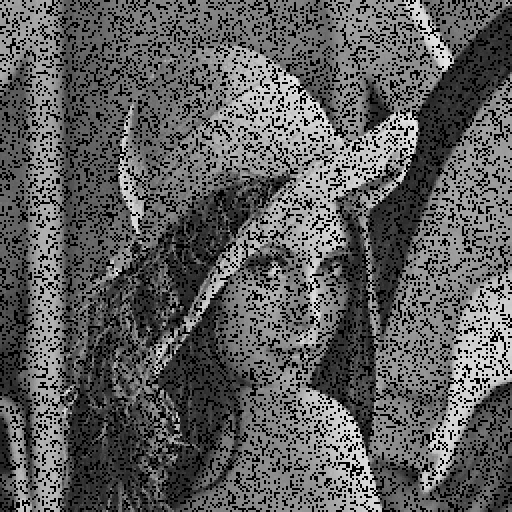
\includegraphics[width=\textwidth]{Chapter5/Images/lenna_haar1.png}
    \caption{Scale 1: PSNR = 11.75}
  \end{subfigure}
  \begin{subfigure}{0.4\textwidth}
    
\includegraphics[width=\textwidth]{Chapter5/Images/lenna_haar2.png}
    \caption{Scale 2: PSNR = 21.78}
  \end{subfigure}
  \begin{subfigure}{0.4\textwidth}
    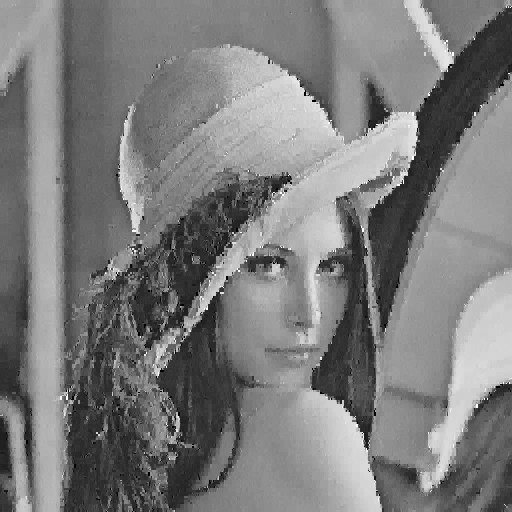
\includegraphics[width=\textwidth]{Chapter5/Images/lenna_haar3.png}
    \caption{Scale 3: PSNR = 24.15}
  \end{subfigure}
  \begin{subfigure}{0.4\textwidth}
    
\includegraphics[width=\textwidth]{Chapter5/Images/lenna_haar4.png}
    \caption{Scale 4: PSNR = 23.72}
  \end{subfigure}  
  \caption[Reconstruction of masked image signals using Haar wavelets at various scales]{Reconstruction if the image in Figure \ref{fig:lenna_mask} using the RVM with Haar wavelets at various scales.
    We use the \emph{Peak Signal-to-Noise Ratio (PSNR)} (see Chapter \ref{ch:results}) as our performance metric. The larger the PSNR, the more accurate the reconstruction.}
  \label{fig:lenna_rvm}
\end{figure}

We see that the scale of the wavelet basis has a strong effect on the quality of the reconstruction.
Wavelets at lower scales can fail to reconstruct the entire image, but generally give a more accurate reconstruction at the portion of the image where they succeed.
On the other, wavelets at larger scales typically achieve a reconstruction of the entire image at the cost of increased blurring or pixelation.
This conflict can be seen in Figure \ref{fig:lenna_rvm} by contrasting panel (c) with panel (d):
They both achieve a reconstruction of the entire image, but scale 3 outperforms scale 4 in this example.
Moreover, if we compare panel (b) with panel (d), we see that, in the part of the image where the recovery succeeds, the scale 2 reconstruction manages to recover finer details than both scale 3 and scale 4.

To explain why this tradeoff exists, recall that two-dimensional Haar wavelets at scale $s$ have a support of size up to $2^s\times 2^s$.
Thus, at small scales, the support of the individual basis functions is small.
For example, suppose $s=1$.
In this case, each Haar basis functions covers an area of $2\times 2$ pixels (see Figure \ref{fig:haar2_basis}).
Using these wavelets, we can capture very local relationships between the pixels.
This allows us to recover finer details in the reconstruction.

However, it can also lead to the formation of black pixels.
At scale 1, each column $j$ of the Haar basis matrix $\bm \Psi$ contains exactly 4 non-zero entries corresponding to the four pixel locations that are covered by the $j$th basis function.
If the masked image happens to be missing data at all four of these locations, the corresponding rows of the basis matrix $\bm\Psi$ will be deleted when forming the design matrix $\bm\Phi=\bm\Theta\bm\Psi$.
Therefore, column $j$ of the design matrix will be zero.
The same is true for the three columns that correspond to the remaining locations that were covered by basis function $j$.

The SSBL algorithm will generally not select any columns that are completely zero, since they offer no change to the marginal likelihood.
The consequence is that the corresponding entries in the posterior mean $\bm\mu$ of $\bm w$ will remain zero.
The resulting reconstruction (\ref{eqn:bcs_recover}) will therefore be unable to recover the $2\times 2$ patch covered by basis function $j$.

This problem can be mitigated by using larger scales since, for any given total number of missing pixels, it is less likely that larger square patches of the masked image are completely void of data.
However, the SSBL Algorithm generally prefers to add basis functions with larger support to the model, since they typically cause a larger increase in the Marginal Likelihood.
The result is that we get a more blurred reconstruction and lose the finer details, even in parts of the image that would have been accurately recovered at smaller scales.





\subsection{Multi-Scale Cascade of Estimations Algorithm}
The \emph{Multi-Scale Cascade of Estimations} (MSCE) algorithm was developed by \cite{pilikos2014} to this tradeoff between inaccurate but complete reconstructions and accurate but incomplete reconstructions.

To explain the algorithm, note that, in the interpolation problem, the BCS reconstruction (\ref{eqn:bcs_recover}) is equivalent to computing the mean (\ref{rvm:pred_mean}) of the predictive distribution (\ref{rvm:predictive}) of the entire signal $\bm v$.
Moreover, we can compute the predictive variance (\ref{rvm:pred_var}) (or error-bars) for each estimate:
\begin{equation}
\label{eqn:msce_error}
  (\sigma^2)^* = \sigma^2 +\bm\psi(\bm x^*)^T\bm\Sigma\bm\psi(\bm x).
\end{equation}

The MSCE algorithm uses these error bars to construct a cascade of BCS algorithms, that builds up the scale of the Haar wavelets.

We begin by executing the BCS algorithm using Haar wavelets at the first scale.
Next, we compute equation (\ref{eqn:msce_error}) for each location in the signal in which originally had missing data.
If $(\sigma^2)^*$ is small, but larger than the noise variance $\sigma^2$, we trust the estimate and accept it. 
If $(\sigma^2)^*$ is large, we do not trust the estimate and reject it.

If $(\sigma^2)^*$ is equal to $\sigma^2$, then $\bm\psi(\bm x^*)^T\bm\Sigma\bm\psi(\bm x^*) = 0$. 
This means that $\bm\psi(\bm x^*) = 0$ since, by postive definiteness of $\bm\Sigma$, $\bm\psi(\bm x^*)^T\bm\Sigma\bm\psi(\bm x^*) > 0$ unless $\bm\psi(\bm x^*) = 0$.
Thus, the RVM predicted the pixel value at location $\bm x^*$ to be zero. 
Since the recovery of the pixel was unsuccessful in this case, we reject the estimate.

The output of the current cascade becomes the target vector of the next cascade.
The new basis matrix is constructed using Haar wavelets that are one scale higher than in the previous cascade.

This process it repeated until we no more signal values marked as missing, or until some pre-defined maximum for the scale of the Haar basis is reached.

We have summarized the MCSE in Algorithm \ref{alg3}.

\begin{algorithm}
  \caption{Multi-Scale Cascade of Estimations \cite{pilikos2014}}
  \label{alg3}
  \begin{algorithmic}[1]
    \State Set $s=1$
    \State Let $\bm y_1 = \bm y$
    \While {$s \leq s_{max}$}
    \State Form basis matrix $\bm\Psi$ using Haar wavelets at scale $s$
    \State Call Sequential Sparse Bayesian Learning Algorithm with target
    \Statex $\qquad$ vector $\bm y_j$ and design matrix $\bm\Phi=\bm\Theta\bm\Psi$ to get the estimate $\bm{\hat v}_s$
    \State Compute $(\sigma^2)^*$ for all newly reconstructed pixel values using equation (\ref{eqn:msce_error})
    \State If $(\sigma^2)^* = \sigma^2$ or $(\sigma^2)^* > \tau$, discard the corresponding estimate
    \State Set $s = s+1$
    \State Let $\bm y_s$ be $\bm{\hat v}_s$ after the discarded estimates are deleted
    \EndWhile
    \State\Return $\bm v = \bm y_s$
  \end{algorithmic}
\end{algorithm}

Note that in practice, we often choose to keep any estimate for which $(\sigma^2)^*>\sigma^2$, so that any prediction that is not zero is trusted.
\chapter{Implementation Details}
\label{ch:code}
We have implemented the MSCE Algorithm for video signals in C++.

In this chapter, we will discuss some of the design decisions and optimizations that went into the implementation.

\section{Blockwise Reconstruction}
Let $\bm v$ be a video signal consisting of $f$ frames with a width of $w$ and a height $h$.
Vectorizing $\bm v$ gives us a vector of length $hwf$.
In order to reconstruct such signals in the Bayesian Compressive Sensing framework (Chapter \ref{ch:msce}), we need to form the basis matrix $\bm\Psi$ which has dimensions $(hwf)\times (hwf)$.

Even for relatively small videos, the memory requirements for such large basis matrices can easily be in the order of terabytes.
As an example, consider the commonly used \emph{CIF (Common Intermediate Format)}.
CIF videos have a spatial resolution of $352 \times 288$.
For a CIF video containing 100 frames, the required memory for storing $\bm\Psi$ as \emph{floats} is 
\begin{equation*}
(288\times 352\times 100)^2 \times 4 \mbox{ bytes} = 4.11 \times 10^{14} \mbox{ bytes} = 411 \mbox{ TB}
\end{equation*}

In our code, we address the problem by performing a \emph{blockwise reconstruction}.
We split the input signal into small sub-blocks of size $2^{j_1}\times 2^{j_2}\times 2^{j_3}$.
A typical size of such a block is $16\times 16\times 16$ (a so-called ``macroblock'').

The blocks are sequentially passed to the MSCE algorithm and after each block has been reconstructed , we put them back together to obtained the recovered video.

Note that the size of the block restricts the number of cascades in the MSCE algorithm.
To run the algorithm up to scale $s$, we require a block size of at least $2^s\times 2^s\times 2^s$.

\section{Code Optimization}
\subsection{Parallelization}
In the blockwise reconstruction, each block is processed independently from the others.
Therefore, we have added an option to the code to process the blocks in parallel.
Using the \emph{Message Passing Interface} (MPI), we run the program on several processors, splitting the workload evenly between them. This generally leads to a very significant speedup.

However, if the blocksize is too small, the communication between processes - when gathering the results - will dominate over the actual computation time.
Initial tests seem to indicate that, in order to achieve a significant increase in the execution time, the blocks should be at least of size $4\times4\times4$ before switching to parallel mode.


\subsection{Fixed Noise Variance}
At each stage of the MSCE algorithm, we keep the noise variance $\sigma^2$ fixed, while training the Sparse Bayesian Learning model.
As noted in Section \ref{sect:ssbl}, doing so allows us to use the efficient update formulae in \cite{tipping2003} which speed up training.

\subsection{Modified RVM Training}
In the MSCE, the RVM is trained using Algorithm \ref{rvm:alg2}.
We use a slightly modified version of the training algorithm in which we only consider addition of basis functions to the model.

At each iteration, we add the basis vector $\bm\phi$ that results in the largest increase of the marginal likelihood.
We continue to do so until none of the remaining candidate basis functions cause an increase in log marginal likelihood that is above the convergence threshold.

For the problem of image and video reconstruction, this modified algorithm gives qualitatively similar results to the unmodified version \cite{pilikos2014}. However, it can lead to a significant reduction in the runtime of the algorithm.


\chapter{Simulations}
\label{ch:results}

\section{Performance Metrics}
In this section, we will introduce three performance metrics that are often used to measure the quality of reconstructed images and videos.

Let $\bm{\hat v} \in\mathbb{R}^M$ be a reconstructed signal (in vectorized form) and let $\bm v$ be the corresponding orginal signal.
The \emph{mean square error} (MSE) of the reconstruction is defined as
\begin{equation*}
  \mse(\bm{\hat v}) = \frac{\sum_{i=1}^M (\hat v_i - v_i)^2}{M}
\end{equation*}
The MSE is zero if and only if we $\bm{\hat v}$ is an exact reconstruction of $\bm v$.

Using the MSE, we can compute the \emph{Peak Signal-to-Noise Ratio} (PSNR) of the reconstruction:
\begin{equation*}
  \psnr(\bm{\hat v}) = 10 \cdot \log_{10} \left(\frac{R^2}{\mse(\bm{\hat v})}\right)
\end{equation*}
where $R$ is the maximum fluctuation in the input signal data type. 
For grayscale images or videos in which the pixel values are stored as 8-bit unsigned integers, we have that $R = 256$.

The PSNR is usually expressed in term of decibel (dB). 
Higher values of the PSNR correspond to more accurate reconstructions.
The PSNR is widely used in the image and video compression literature to measure the quality of a compressed signal.
Generally, when comparing the reconstruction quality, the PSNR should only be used if it was measured on the same signal.

The final performance metric that we compute is the \emph{relative reconstruction error}.
It is given by
\begin{equation*}
  \rre(\bm{\hat v}) = \frac{||\bm{\hat v} - \bm v||_2}{||\bm v||_2}
\end{equation*}
This is the metric that was used in \cite{ji2008} and \cite{pilikos2014}.

\section{Experiments}
In this section, we perform experiments in order to get an idea of how the different components of the implementation perform.
All simulations were run on the ``foreman'' test video using blocks of size $8\times 8\times 8$.

\subsection{MSCE vs BCS}
We compare the performance of using cascades over individual BCS

\subsection{DCT vs Haar(3)}
In Figure \ref{fig:sim_basis}, we compareshows a comparison between using the DCT basis and the Haar basis.

\subsection{Gaussan vs Bernoulli vs Mask}
We compare 

\subsection{Haar Scales with Gaussian \texorpdfstring{$\bm\Theta$}{[Theta]}}

%% CASCADE
\begin{figure}
  \centering
  \begin{tikzpicture}[scale = 0.8,baseline]
    \begin{axis}[
      xlabel=$N/M$ (\%),
      ylabel=$\rre$ (\%),
      xmin=0, xmax = 100,
      ymin = 0, ymax = 0.2,
      scaled ticks=false,
      yticklabel style={
        /pgf/number format/precision=2,
        /pgf/number format/fixed,
      }
      ]
      \addplot table [x=pc, y=rre] {Chapter7/Images/MSCE.dat};      
      \addlegendentry{MSCE}
      \addplot table [x=pc, y=rre] {Chapter7/Images/MASK_3.dat};      
      \addlegendentry{BCS Scale 3}
      \addplot table [x=pc, y=rre] {Chapter7/Images/MASK_2.dat};     
      \addlegendentry{BCS Scale 2}
      \addplot table [x=pc, y=rre] {Chapter7/Images/MASK_1.dat};
      \addlegendentry{BCS Scale 1}
    \end{axis}
  \end{tikzpicture}
  % 
  \hskip 10pt
  % 
  \begin{tikzpicture}[scale = 0.8,baseline]
    \begin{axis}[
      xlabel=$N/M$ (\%),
      ylabel=$\psnr$ (dB),
      xmin=0, xmax = 90, 
      scaled ticks=false,
      legend style={
        at={(0.03,1.04)},
        anchor=north west,
      },
      yticklabel style={
        /pgf/number format/precision=2,
        /pgf/number format/fixed,
      }
      ]
      \addplot table [x=pc, y=psnr] {Chapter7/Images/MSCE.dat};      
      \addlegendentry{MSCE}
      \addplot table [x=pc, y=psnr] {Chapter7/Images/MASK_3.dat};
      \addlegendentry{BCS Scale 3}
      \addplot table [x=pc, y=psnr] {Chapter7/Images/MASK_2.dat};
      \addlegendentry{BCS Scale 2}
      \addplot table [x=pc, y=psnr] {Chapter7/Images/MASK_1.dat};
      \addlegendentry{BCS Scale 1}
    \end{axis}
  \end{tikzpicture}
\caption{Performance of MSCE with 3 cascades and uniform Masks}
\label{fig:sim_msce}
\end{figure}

%% BASIS
\begin{figure}
  \centering
  \begin{tikzpicture}[scale = 0.8,baseline]
    \begin{axis}[
      xlabel=$N/M$ (\%),
      ylabel=$\rre$ (\%),
      xmin=0, xmax = 100,
      ymin = 0, 
      scaled ticks=false,
      yticklabel style={
        /pgf/number format/precision=2,
        /pgf/number format/fixed,
      }
      ]
      \addplot table [x=pc, y=rre] {Chapter7/Images/GAUSS_DCT.dat};      
      \addlegendentry{DCT}
      \addplot table [x=pc, y=rre] {Chapter7/Images/GAUSS_HAAR.dat};      
      \addlegendentry{Haar}
    \end{axis}
  \end{tikzpicture}
  % 
  \hskip 10pt
  % 
  \begin{tikzpicture}[scale = 0.8,baseline]
    \begin{axis}[
      xlabel=$N/M$ (\%),
      ylabel=$\psnr$ (dB),
      xmin=0, xmax = 90,      
      scaled ticks=false,
      legend style={
        at={(0.03,0.98)},
        anchor=north west,
      },
      yticklabel style={
        /pgf/number format/precision=2,
        /pgf/number format/fixed,
      }
      ]
      \addplot table [x=pc, y=psnr] {Chapter7/Images/GAUSS_DCT.dat};      
      \addlegendentry{DCT}
      \addplot table [x=pc, y=psnr] {Chapter7/Images/GAUSS_HAAR.dat};      
      \addlegendentry{Haar}
    \end{axis}
  \end{tikzpicture}
\caption{DCT vs Haar DWT (scale 3) with Gaussian measurements}
\label{fig:sim_basis}
\end{figure}

%% SENSORS
\begin{figure}
  \centering
  \begin{tikzpicture}[scale = 0.8,baseline]
    \begin{axis}[
      xlabel=$N/M$ (\%),
      ylabel=$\rre$ (\%),
      xmin=0, xmax = 100,
      ymin = 0, 
      scaled ticks=false,
      yticklabel style={
        /pgf/number format/precision=2,
        /pgf/number format/fixed,
      }
      ]
      \addplot table [x=pc, y=rre] {Chapter7/Images/GAUSS_DCT.dat};      
      \addlegendentry{Gauss}
      \addplot table [x=pc, y=rre] {Chapter7/Images/BERN_DCT.dat};      
      \addlegendentry{Bernoulli}
      \addplot table [x=pc, y=rre] {Chapter7/Images/MASK_DCT.dat};      
      \addlegendentry{Mask}
    \end{axis}
  \end{tikzpicture}
  % 
  \hskip 10pt
  % 
  \begin{tikzpicture}[scale = 0.8,baseline]
    \begin{axis}[
      xlabel=$N/M$ (\%),
      ylabel=$\psnr$ (dB),
      xmin=0, xmax = 90,      
      scaled ticks=false,
      legend style={
        at={(0.03,0.98)},
        anchor=north west,
      },
      yticklabel style={
        /pgf/number format/precision=2,
        /pgf/number format/fixed,
      }
      ]
      \addplot table [x=pc, y=psnr] {Chapter7/Images/GAUSS_DCT.dat};      
      \addlegendentry{Gauss}
      \addplot table [x=pc, y=psnr] {Chapter7/Images/BERN_DCT.dat};      
      \addlegendentry{Bernoulli}
      \addplot table [x=pc, y=psnr] {Chapter7/Images/MASK_DCT.dat};      
      \addlegendentry{Mask}
    \end{axis}
  \end{tikzpicture}
\caption{Gaussian vs Bernoulli vs Mask (uniform) with DCT basis}
\label{fig:sim_sensor}
\end{figure}

%% SCALES
\begin{figure}
  \centering
  \begin{tikzpicture}[scale = 0.8,baseline]
    \begin{axis}[
      xlabel=$N/M$ (\%),
      ylabel=$\rre$ (\%),
      xmin=0, xmax = 100,
      ymin = 0, 
      scaled ticks=false,
      yticklabel style={
        /pgf/number format/precision=2,
        /pgf/number format/fixed,
      }
      ]
      \addplot table [x=pc, y=rre] {Chapter7/Images/HAAR_GAUSS_1.dat};      
      \addlegendentry{Scale 1}
      \addplot table [x=pc, y=rre] {Chapter7/Images/HAAR_GAUSS_2.dat};
      \addlegendentry{Scale 2}
      \addplot table [x=pc, y=rre] {Chapter7/Images/HAAR_GAUSS_3.dat};
      \addlegendentry{Scale 3}
    \end{axis}
  \end{tikzpicture}
  % 
  \hskip 10pt
  % 
  \begin{tikzpicture}[scale = 0.8,baseline]
    \begin{axis}[
      xlabel=$N/M$ (\%),
      ylabel=$\psnr$ (dB),
      xmin=0, xmax = 90,      
      scaled ticks=false,
      legend style={
        at={(0.03,0.98)},
        anchor=north west,
      },
      yticklabel style={
        /pgf/number format/precision=2,
        /pgf/number format/fixed,
      }
      ]
      \addplot table [x=pc, y=psnr] {Chapter7/Images/HAAR_GAUSS_1.dat};
      \addlegendentry{Scale 1}
      \addplot table [x=pc, y=psnr] {Chapter7/Images/HAAR_GAUSS_2.dat};
      \addlegendentry{Scale 2}
      \addplot table [x=pc, y=psnr] {Chapter7/Images/HAAR_GAUSS_3.dat};
      \addlegendentry{Scale 3}
    \end{axis}
  \end{tikzpicture}
\caption{Haar wavelets at different scales with Gaussian measurements (fixed block size)}
\label{fig:sim_scales}
\end{figure}

\clearpage

\section{Example Results}

\begin{figure}[!ht]
  \centering
  \textbf{\hspace{0.2in} Frame 2 \hspace{1.5in} Frame 19\hspace{0.5in}\vspace{0.2in}}
  \begin{subfigure}{0.4\textwidth}
    \centering
    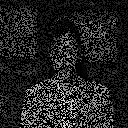
\includegraphics[width=0.8\textwidth]{Chapter7/Images/akiyo40_masked_2.png}
    \caption{Corrupted}
  \end{subfigure}
  \begin{subfigure}{0.4\textwidth}
    \centering
    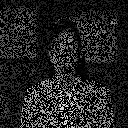
\includegraphics[width=0.8\textwidth]{Chapter7/Images/akiyo40_masked_19.png}
    \caption{Corrupted}
  \end{subfigure}
  \begin{subfigure}{0.4\textwidth}
    \centering
    
\includegraphics[width=0.8\textwidth]{Chapter7/Images/akiyo40_rec_2.png}
    \caption{Recovered}
  \end{subfigure}
  \begin{subfigure}{0.4\textwidth}
    \centering
    
\includegraphics[width=0.8\textwidth]{Chapter7/Images/akiyo40_rec_19.png}
    \caption{Recovered}
  \end{subfigure}
  \begin{subfigure}{0.4\textwidth}
    \centering
    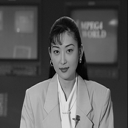
\includegraphics[width=0.8\textwidth]{Chapter7/Images/akiyo40_orig_2.png}
    \caption{Original}
  \end{subfigure}
  \begin{subfigure}{0.4\textwidth}
    \centering
    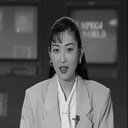
\includegraphics[width=0.8\textwidth]{Chapter7/Images/akiyo40_orig_19.png}
    \caption{Original}
  \end{subfigure}
  \caption{Reconstruction of $128\times 128\times 128$ video signal ``akiyo'' from 40\% of the measurement using the MSCE with 3 cascades. Mask decimation pattern is uniform. $\psnr = 30.02$}
\end{figure}

\begin{figure}
  \centering
  \textbf{\hspace{0.2in} Frame 32 \hspace{1.5in} Frame 52\hspace{0.5in}\vspace{0.1in}}
  \begin{subfigure}{0.4\textwidth}
    \centering
    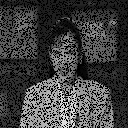
\includegraphics[width=0.9\textwidth]{Chapter7/Images/akiyo70_masked_32.png}
    \caption{Corrupted}
  \end{subfigure}
  \begin{subfigure}{0.4\textwidth}
    \centering
    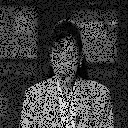
\includegraphics[width=0.9\textwidth]{Chapter7/Images/akiyo70_masked_52.png}
    \caption{Corrupted}
  \end{subfigure}
  \begin{subfigure}{0.4\textwidth}
    \centering
    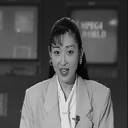
\includegraphics[width=.9\textwidth]{Chapter7/Images/akiyo70_rec_32.png}
    \caption{Recovered}
  \end{subfigure}
  \begin{subfigure}{0.4\textwidth}
    \centering
    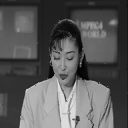
\includegraphics[width=.9\textwidth]{Chapter7/Images/akiyo70_rec_52.png}
    \caption{Recovered}
  \end{subfigure}
  \begin{subfigure}{0.4\textwidth}
    \centering
    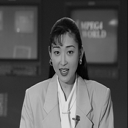
\includegraphics[width=.9\textwidth]{Chapter7/Images/akiyo70_orig_32.png}
    \caption{Original}
  \end{subfigure}
  \begin{subfigure}{0.4\textwidth}
    \centering
    
\includegraphics[width=.9\textwidth]{Chapter7/Images/akiyo70_orig_52.png}
    \caption{Original}
  \end{subfigure}
  \caption{Reconstruction of $128\times 128\times 128$ video signal ``akiyo'' from 70\% of the measurement using the MSCE with 3 cascades. Mask decimation pattern is uniform. $\psnr = 36.86$}
\end{figure}

\begin{figure}
  \centering
  \textbf{\hspace{0.2in} Frame 18 \hspace{1.5in} Frame 22\hspace{0.5in}\vspace{0.1in}}
  \begin{subfigure}{0.4\textwidth}
    \centering
    
\includegraphics[width=.9\textwidth]{Chapter7/Images/foreman40_masked_18.png}
    \caption{Corrupted}
  \end{subfigure}
  \begin{subfigure}{0.4\textwidth}
    \centering
    
\includegraphics[width=.9\textwidth]{Chapter7/Images/foreman40_masked_22.png}
    \caption{Corrupted}
  \end{subfigure}
  \begin{subfigure}{0.4\textwidth}
    \centering
    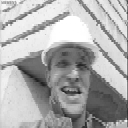
\includegraphics[width=.9\textwidth]{Chapter7/Images/foreman40_rec_18.png}
    \caption{Recovered}
  \end{subfigure}
  \begin{subfigure}{0.4\textwidth}
    \centering
    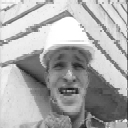
\includegraphics[width=.9\textwidth]{Chapter7/Images/foreman40_rec_22.png}
    \caption{Recovered}
  \end{subfigure}
  \begin{subfigure}{0.4\textwidth}
    \centering
    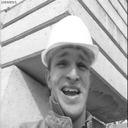
\includegraphics[width=.9\textwidth]{Chapter7/Images/foreman40_orig_18.png}
    \caption{Original}
  \end{subfigure}
  \begin{subfigure}{0.4\textwidth}
    \centering
    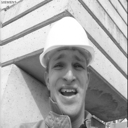
\includegraphics[width=.9\textwidth]{Chapter7/Images/foreman40_orig_22.png}
    \caption{Original}
  \end{subfigure}
  \caption{Reconstruction of $128\times 128\times 128$ video signal ``foreman'' from 40\% of the measurement using the MSCE with 3 cascades. Mask decimation pattern is: horizontal lines that are randomly generated for each frame. $\psnr = 25.50$}
\end{figure}


\begin{figure}
  \centering
  \textbf{\hspace{0.2in} Frame 18 \hspace{1.5in} Frame 22\hspace{0.5in}\vspace{0.1in}}
  \begin{subfigure}{0.4\textwidth}
    \centering
    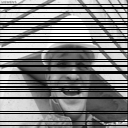
\includegraphics[width=.9\textwidth]{Chapter7/Images/foreman70_masked_18.png}
    \caption{Corrupted}
  \end{subfigure}
  \begin{subfigure}{0.4\textwidth}
    \centering
    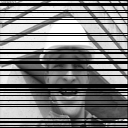
\includegraphics[width=.9\textwidth]{Chapter7/Images/foreman70_masked_22.png}
    \caption{Corrupted}
  \end{subfigure}
  \begin{subfigure}{0.4\textwidth}
    \centering
    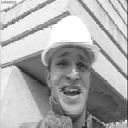
\includegraphics[width=.9\textwidth]{Chapter7/Images/foreman70_rec_18.png}
    \caption{Recovered}
  \end{subfigure}
  \begin{subfigure}{0.4\textwidth}
    \centering
    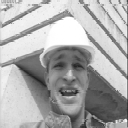
\includegraphics[width=.9\textwidth]{Chapter7/Images/foreman70_rec_22.png}
    \caption{Recovered}
  \end{subfigure}
  \begin{subfigure}{0.4\textwidth}
    \centering
    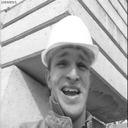
\includegraphics[width=.9\textwidth]{Chapter7/Images/foreman70_orig_18.png}
    \caption{Original}
  \end{subfigure}
  \begin{subfigure}{0.4\textwidth}
    \centering
    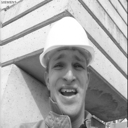
\includegraphics[width=.9\textwidth]{Chapter7/Images/foreman70_orig_22.png}
    \caption{Original}
  \end{subfigure}
  \caption{Reconstruction of $128\times 128\times 128$ video signal ``foreman'' from 70\% of the measurement using the MSCE with 3 cascades. Mask decimation pattern is: horizontal lines that are randomly generated for each frame. $\psnr = 30.32$}
\end{figure}

\begin{figure}
  \centering
  \textbf{\hspace{0.2in} Frame 11 \hspace{1.5in} Frame 12\hspace{0.5in}\vspace{0.1in}}
  \begin{subfigure}{0.4\textwidth}
    \centering
    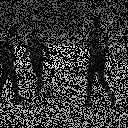
\includegraphics[width=.9\textwidth]{Chapter7/Images/soccer40_masked_11.png}
    \caption{Corrupted}
  \end{subfigure}
  \begin{subfigure}{0.4\textwidth}
    \centering
    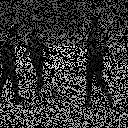
\includegraphics[width=.9\textwidth]{Chapter7/Images/soccer40_masked_12.png}
    \caption{Corrupted}
  \end{subfigure}
  \begin{subfigure}{0.4\textwidth}
    \centering
    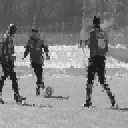
\includegraphics[width=.9\textwidth]{Chapter7/Images/soccer40_rec_11.png}
    \caption{Recovered}
  \end{subfigure}
  \begin{subfigure}{0.4\textwidth}
    \centering
    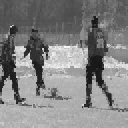
\includegraphics[width=.9\textwidth]{Chapter7/Images/soccer40_rec_12.png}
    \caption{Recovered}
  \end{subfigure}
  \begin{subfigure}{0.4\textwidth}
    \centering
    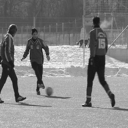
\includegraphics[width=.9\textwidth]{Chapter7/Images/soccer40_orig_11.png}
    \caption{Original}
  \end{subfigure}
  \begin{subfigure}{0.4\textwidth}
    \centering
    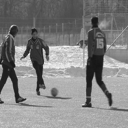
\includegraphics[width=.9\textwidth]{Chapter7/Images/soccer40_orig_12.png}
    \caption{Original}
  \end{subfigure}
  \caption{Reconstruction of $128\times 128\times 128$ video signal ``soccer'' from 40\% of the measurement using the MSCE with 3 cascades. Mask decimation pattern is: missing pixels that are constant across the frames. $\psnr = 24.84$}
\end{figure}



\begin{figure}
  \centering
  \textbf{\hspace{0.2in} Frame 11 \hspace{1.5in} Frame 12\hspace{0.5in}\vspace{0.1in}}
  \begin{subfigure}{0.4\textwidth}
    \centering
    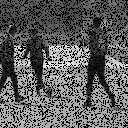
\includegraphics[width=.9\textwidth]{Chapter7/Images/soccer70_masked_11.png}
    \caption{Corrupted}
  \end{subfigure}
  \begin{subfigure}{0.4\textwidth}
    \centering
    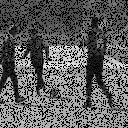
\includegraphics[width=.9\textwidth]{Chapter7/Images/soccer70_masked_12.png}
    \caption{Corrupted}
  \end{subfigure}
  \begin{subfigure}{0.4\textwidth}
    \centering
    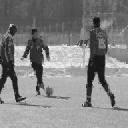
\includegraphics[width=.9\textwidth]{Chapter7/Images/soccer70_rec_11.png}
    \caption{Recovered}
  \end{subfigure}
  \begin{subfigure}{0.4\textwidth}
    \centering
    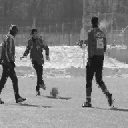
\includegraphics[width=.9\textwidth]{Chapter7/Images/soccer70_rec_12.png}
    \caption{Recovered}
  \end{subfigure}
  \begin{subfigure}{0.4\textwidth}
    \centering
    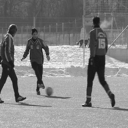
\includegraphics[width=.9\textwidth]{Chapter7/Images/soccer70_orig_11.png}
    \caption{Original}
  \end{subfigure}
  \begin{subfigure}{0.4\textwidth}
    \centering
    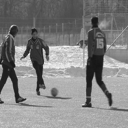
\includegraphics[width=.9\textwidth]{Chapter7/Images/soccer70_orig_12.png}
    \caption{Original}
  \end{subfigure}
  \caption{Reconstruction of $128\times 128\times 128$ video signal ``soccer'' from 70\% of the measurement using the MSCE with 3 cascades. Mask decimation pattern is: missing pixels that are constant across the frames. $\psnr = 29.35$}
\end{figure}

\begin{figure}
  \centering
  \textbf{\hspace{0.5in} Frame 21 \hspace{1.5in} Frame 151\hspace{0.5in}\vspace{0.2in}}
  \begin{subfigure}{0.4\textwidth}
    
\includegraphics[width=\textwidth]{Chapter5/Images/foreman_masked_21.png}
    \caption{Corrupted}
  \end{subfigure}
  \begin{subfigure}{0.4\textwidth}
    \includegraphics[width=\textwidth]{Chapter5/Images/foreman_masked_151.png}
    \caption{Corrupted}
  \end{subfigure}
  \begin{subfigure}{0.4\textwidth}
    \includegraphics[width=\textwidth]{Chapter5/Images/foreman_rec_21.png}
    \caption{Recovered}
  \end{subfigure}
  \begin{subfigure}{0.4\textwidth}
    \includegraphics[width=\textwidth]{Chapter5/Images/foreman_rec_151.png}
    \caption{Recovered}
  \end{subfigure}
  \begin{subfigure}{0.4\textwidth}
    \includegraphics[width=\textwidth]{Chapter5/Images/foreman_orig_21.png}
    \caption{Original}
  \end{subfigure}
  \begin{subfigure}{0.4\textwidth}
    \includegraphics[width=\textwidth]{Chapter5/Images/foreman_orig_151.png}
    \caption{Original}
  \end{subfigure}
  \caption[Example output of our video interpolator]{Example of a masked video signal, where only 60\% of the pixel values are known (a-b). 
    Reconstruction via the MSCE Algorithm using 2 cascades (PSNR: 28.6) (c-d).
    Original video (e-f).}
  \label{fig:foreman_masked}
\end{figure}

\chapter{Conclusion}
\label{ch:conclusion}

For the MPhil thesis, we set out to develop a generic Compressive Sensing algorithm that provides high quality reconstructions of video signals from relatively small numbers of samples.


In this thesis, we investigated the efficacy of the Bayesian Compressive Sensing framework for efficient reconstruction of highly under-sampled video signals.
We developed an extension to the Multi-Scale Cascade of Estimations algorithm that achieves near-perfect reconstructions of videos from a very small set of measurements.

To do so, we constructed three-dimensional wavelet basis functions that allow for a highly compressible representation of the video signal.
Compressive Sensing inversion is then formulated as a machine learning problem and the Relevance Vector Machine was employed to find highly sparse solutions.
To boost performance, a cascade of RVMs it built that exploits the multi-resolution properties of wavelet basis functions.

In order to deal with the large memory requirements of the algorithm, the reconstruction is performed in blockwise fashion.
We have also implemented the method as a distributed program, resulting in dramatically reduced execution times.

Future research could improve performance by extending these methods in various ways.
In order to fully harness the power of the MSCE for video interpolation, the implentation should be extended to accommodate different kinds of wavelets.
Using the simple Haar wavelets, the MSCE struggles to outperform a BCT that uses DCT basis functions.
It only shows its advantage in extremely undersampled situations ($N < 0.2M$).
Alternative sets of waveles, such as the CDF-9/7 wavelet that is used by the JPEG2000 format, may lead to sparser representations of the video signals. 

Furthermore, the speed of the algorithm can be increased by using a multi-threaded implementation of the Sequential Sparse Bayesian Learning Algorithm. 

Development of Bayesian approaches to Compressive Sensing systems is an active area of research.


%\include{Chapter9/chapter9}



% ********************************** Back Matter *******************************
% Backmatter should be commented out, if you are using appendices after References
%\backmatter

% ********************************** Bibliography ******************************
\begin{spacing}{0.9}

% To use the conventional natbib style referencing
% Bibliography style previews: http://nodonn.tipido.net/bibstyle.php
% Reference styles: http://sites.stat.psu.edu/~surajit/present/bib.htm

\bibliographystyle{apalike}
%\bibliographystyle{plainnat} % use this to have URLs listed in References
\cleardoublepage
\bibliography{References/references} % Path to your References.bib file


% If you would like to use BibLaTeX for your references, pass `custombib' as
% an option in the document class. The location of 'reference.bib' should be
% specified in the preamble.tex file in the custombib section.
% Comment out the lines related to natbib above and uncomment the following line.

%\printbibliography[heading=bibintoc, title={References}]


\end{spacing}

% ********************************** Appendices ********************************

\begin{appendices} % Using appendices environment for more functunality

% % ******************************* Thesis Appendix A ********************************
\chapter{How to install \LaTeX} 

\section*{Windows OS}

\subsection*{TeXLive package - full version}
\begin{enumerate}
\item	Download the TeXLive ISO (2.2GB) from\\
\href{https://www.tug.org/texlive/}{https://www.tug.org/texlive/}
\item	Download WinCDEmu (if you don't have a virtual drive) from \\
\href{http://wincdemu.sysprogs.org/download/}{http://wincdemu.sysprogs.org/download/}
\item	To install Windows CD Emulator follow the instructions at\\
\href{http://wincdemu.sysprogs.org/tutorials/install/}{http://wincdemu.sysprogs.org/tutorials/install/}
\item	Right click the iso and mount it using the WinCDEmu as shown in \\
\href{http://wincdemu.sysprogs.org/tutorials/mount/}{http://wincdemu.sysprogs.org/tutorials/mount/}
\item	Open your virtual drive and run setup.pl
\end{enumerate}

or

\subsection*{Basic MikTeX - TeX distribution}
\begin{enumerate}
\item	Download Basic-MiK\TeX (32bit or 64bit) from\\
\href{http://miktex.org/download}{http://miktex.org/download}
\item	Run the installer 
\item	To add a new package go to Start >> All Programs >> MikTex >> Maintenance (Admin) and choose Package Manager
\item	Select or search for packages to install
\end{enumerate}

\subsection*{TexStudio - Tex Editor}
\begin{enumerate}
\item	Download TexStudio from\\
\href{http://texstudio.sourceforge.net/\#downloads}{http://texstudio.sourceforge.net/\#downloads} 
\item	Run the installer
\end{enumerate}

\section*{Mac OS X}
\subsection*{MacTeX - TeX distribution}
\begin{enumerate}
\item	Download the file from\\
\href{https://www.tug.org/mactex/}{https://www.tug.org/mactex/}
\item	Extract and double click to run the installer. It does the entire configuration, sit back and relax.
\end{enumerate}

\subsection*{TexStudio - Tex Editor}
\begin{enumerate}
\item	Download TexStudio from\\
\href{http://texstudio.sourceforge.net/\#downloads}{http://texstudio.sourceforge.net/\#downloads} 
\item	Extract and Start
\end{enumerate}


\section*{Unix/Linux}
\subsection*{TeXLive - TeX distribution}
\subsubsection*{Getting the distribution:}
\begin{enumerate}
\item	TexLive can be downloaded from\\
\href{http://www.tug.org/texlive/acquire-netinstall.html}{http://www.tug.org/texlive/acquire-netinstall.html}.
\item	TexLive is provided by most operating system you can use (rpm,apt-get or yum) to get TexLive distributions
\end{enumerate}

\subsubsection*{Installation}
\begin{enumerate}
\item	Mount the ISO file in the mnt directory
\begin{verbatim}
mount -t iso9660 -o ro,loop,noauto /your/texlive####.iso /mnt
\end{verbatim}

\item	Install wget on your OS (use rpm, apt-get or yum install)
\item	Run the installer script install-tl.
\begin{verbatim}
	cd /your/download/directory
	./install-tl
\end{verbatim}
\item	Enter command `i' for installation

\item	Post-Installation configuration:\\
\href{http://www.tug.org/texlive/doc/texlive-en/texlive-en.html\#x1-320003.4.1}{http://www.tug.org/texlive/doc/texlive-en/texlive-en.html\#x1-320003.4.1} 
\item	Set the path for the directory of TexLive binaries in your .bashrc file
\end{enumerate}

\subsubsection*{For 32Bit OS}
For Bourne-compatible shells such as bash, and using Intel x86 GNU/Linux and a default directory setup as an example, the file to edit might be \begin{verbatim}
edit $~/.bashrc file and add following lines
PATH=/usr/local/texlive/2011/bin/i386-linux:$PATH; 
export PATH 
MANPATH=/usr/local/texlive/2011/texmf/doc/man:$MANPATH;
export MANPATH 
INFOPATH=/usr/local/texlive/2011/texmf/doc/info:$INFOPATH;
export INFOPATH
\end{verbatim}
\subsubsection*{For 64Bit}
\begin{verbatim}
edit $~/.bashrc file and add following lines
PATH=/usr/local/texlive/2011/bin/x86_64-linux:$PATH;
export PATH 
MANPATH=/usr/local/texlive/2011/texmf/doc/man:$MANPATH;
export MANPATH 
INFOPATH=/usr/local/texlive/2011/texmf/doc/info:$INFOPATH;
export INFOPATH

\end{verbatim}



%\subsection{Installing directly using Linux packages} 
\subsubsection*{Fedora/RedHat/CENTOS:}
\begin{verbatim} 
sudo yum install texlive 
sudo yum install psutils 
\end{verbatim}


\subsubsection*{SUSE:}
\begin{verbatim}
sudo zypper install texlive
\end{verbatim}


\subsubsection*{Debian/Ubuntu:}
\begin{verbatim} 
sudo apt-get install texlive texlive-latex-extra 
sudo apt-get install psutils
\end{verbatim}

% % ******************************* Thesis Appendix B ********************************

\chapter{Installing the CUED Class file}

\LaTeX.cls files can be accessed system-wide when they are placed in the
<texmf>/tex/latex directory, where <texmf> is the root directory of the user’s \TeX installation. On systems that have a local texmf tree (<texmflocal>), which
may be named ``texmf-local'' or ``localtexmf'', it may be advisable to install packages in <texmflocal>, rather than <texmf> as the contents of the former, unlike that of the latter, are preserved after the \LaTeX system is reinstalled and/or upgraded.

It is recommended that the user create a subdirectory <texmf>/tex/latex/CUED for all CUED related \LaTeX class and package files. On some \LaTeX systems, the directory look-up tables will need to be refreshed after making additions or deletions to the system files. For \TeX Live systems this is accomplished via executing ``texhash'' as root. MIK\TeX users can run ``initexmf -u'' to accomplish the same thing.

Users not willing or able to install the files system-wide can install them in their personal directories, but will then have to provide the path (full or relative) in addition to the filename when referring to them in \LaTeX.



\end{appendices}

% *************************************** Index ********************************
\printthesisindex % If index is present

\end{document}
